\documentclass[11pt]{article}
\usepackage[a4paper,margin=2.4cm]{geometry}
\usepackage[T1]{fontenc}
\usepackage[utf8]{inputenc}
\usepackage{lmodern}
\usepackage{microtype}
\usepackage{amsmath,amssymb}
\usepackage{booktabs}
\usepackage{makecell}
\usepackage{adjustbox}
\usepackage{graphicx}
\usepackage{xcolor}
\usepackage{tikz}
\usetikzlibrary{positioning,arrows.meta,calc}
\usepackage[numbers,sort&compress]{natbib}
\usepackage{setspace}
\usepackage{lineno}
\usepackage[hidelinks]{hyperref}
\usepackage{caption}
\captionsetup{font=small,labelfont=bf}
\newcommand{\authorinput}[1]{\textcolor{red}{\textbf{[#1]}}}

% Every number quoted from the data comes from generated/values.tex (see README.md).
% Generated by careport.psg_assist_manuscript from the committed reports; do not edit.
\expandafter\def\csname val@a1-human-kappa-hi\endcsname{+0.002}
\expandafter\def\csname val@a1-human-kappa-lo\endcsname{\ensuremath{-}0.024}
\expandafter\def\csname val@a1-human-kappa-mean\endcsname{\ensuremath{-}0.010}
\expandafter\def\csname val@a1-human-pct-hi\endcsname{+0.001}
\expandafter\def\csname val@a1-human-pct-lo\endcsname{\ensuremath{-}0.015}
\expandafter\def\csname val@a1-human-pct-mean\endcsname{\ensuremath{-}0.007}
\expandafter\def\csname val@a1-human-share-left\endcsname{61\%}
\expandafter\def\csname val@a1-yasa-kappa-mean\endcsname{\ensuremath{-}0.027}
\expandafter\def\csname val@a1-yasa-kappa-neg\endcsname{4}
\expandafter\def\csname val@a1-yasa-pct-mean\endcsname{\ensuremath{-}0.017}
\expandafter\def\csname val@a1-yasa-pct-neg\endcsname{4}
\expandafter\def\csname val@a1-yasa-share-left\endcsname{67\%}
\expandafter\def\csname val@a1-yasa-sn1-kappa\endcsname{+0.010}
\expandafter\def\csname val@a1-yasa-sn1-pct\endcsname{+0.007}
\expandafter\def\csname val@a1-yasa-sn2-kappa\endcsname{\ensuremath{-}0.027}
\expandafter\def\csname val@a1-yasa-sn2-pct\endcsname{\ensuremath{-}0.021}
\expandafter\def\csname val@a1-yasa-sn3-kappa\endcsname{\ensuremath{-}0.021}
\expandafter\def\csname val@a1-yasa-sn3-pct\endcsname{\ensuremath{-}0.016}
\expandafter\def\csname val@a1-yasa-sn4-kappa\endcsname{\ensuremath{-}0.041}
\expandafter\def\csname val@a1-yasa-sn4-pct\endcsname{\ensuremath{-}0.031}
\expandafter\def\csname val@a1-yasa-sn5-kappa\endcsname{\ensuremath{-}0.055}
\expandafter\def\csname val@a1-yasa-sn5-pct\endcsname{\ensuremath{-}0.024}
\expandafter\def\csname val@a2-arousals-assisted\endcsname{0.788}
\expandafter\def\csname val@a2-arousals-assisted-pct\endcsname{79\%}
\expandafter\def\csname val@a2-arousals-diff\endcsname{+0.575}
\expandafter\def\csname val@a2-arousals-manual\endcsname{0.212}
\expandafter\def\csname val@a2-arousals-n\endcsname{23{,}176}
\expandafter\def\csname val@a2-arousals-rec-max\endcsname{0.76}
\expandafter\def\csname val@a2-arousals-rec-min\endcsname{0.16}
\expandafter\def\csname val@a2-limb-assisted\endcsname{0.988}
\expandafter\def\csname val@a2-limb-assisted-pct\endcsname{99\%}
\expandafter\def\csname val@a2-limb-diff\endcsname{+0.976}
\expandafter\def\csname val@a2-limb-manual\endcsname{0.012}
\expandafter\def\csname val@a2-limb-n\endcsname{11{,}550}
\expandafter\def\csname val@a2-limb-rec-max\endcsname{0.99}
\expandafter\def\csname val@a2-limb-rec-min\endcsname{0.96}
\expandafter\def\csname val@a2-max-pct\endcsname{99\%}
\expandafter\def\csname val@a2-min-pct\endcsname{79\%}
\expandafter\def\csname val@a2-resp-assisted\endcsname{0.951}
\expandafter\def\csname val@a2-resp-assisted-pct\endcsname{95\%}
\expandafter\def\csname val@a2-resp-diff\endcsname{+0.902}
\expandafter\def\csname val@a2-resp-manual\endcsname{0.049}
\expandafter\def\csname val@a2-resp-n\endcsname{27{,}754}
\expandafter\def\csname val@a2-resp-rec-max\endcsname{0.99}
\expandafter\def\csname val@a2-resp-rec-min\endcsname{0.50}
\expandafter\def\csname val@a2-sign-n\endcsname{20}
\expandafter\def\csname val@a2-sign-p\endcsname{\ensuremath{1.9\times10^{-6}}}
\expandafter\def\csname val@a2-sign-pos\endcsname{20}
\expandafter\def\csname val@a2-stages-assisted\endcsname{0.930}
\expandafter\def\csname val@a2-stages-assisted-pct\endcsname{93\%}
\expandafter\def\csname val@a2-stages-diff\endcsname{+0.871}
\expandafter\def\csname val@a2-stages-manual\endcsname{0.058}
\expandafter\def\csname val@a2-stages-n\endcsname{171}
\expandafter\def\csname val@a2-stages-rec-max\endcsname{1.00}
\expandafter\def\csname val@a2-stages-rec-min\endcsname{0.73}
\expandafter\def\csname val@a2-stages-share\endcsname{3.6\%}
\expandafter\def\csname val@a3-arousals-closer\endcsname{1}
\expandafter\def\csname val@a3-limb-closer\endcsname{0}
\expandafter\def\csname val@a3-resp-closer\endcsname{2}
\expandafter\def\csname val@a3-stage-manual\endcsname{0.964}
\expandafter\def\csname val@a3-stage-prefill\endcsname{0.947}
\expandafter\def\csname val@a3-stages-closer\endcsname{3}
\expandafter\def\csname val@a3-units-n\endcsname{20}
\expandafter\def\csname val@a3-units-p\endcsname{0.12}
\expandafter\def\csname val@a3-units-pos\endcsname{6}
\expandafter\def\csname val@b1-gap-d0\endcsname{0.108}
\expandafter\def\csname val@b1-gap-d0-bias\endcsname{+0.059}
\expandafter\def\csname val@b1-gap-d0s\endcsname{0.112}
\expandafter\def\csname val@b1-gap-d0s-bias\endcsname{+0.063}
\expandafter\def\csname val@b1-gap-f1-d1\endcsname{0.117}
\expandafter\def\csname val@b1-gap-f1-d2\endcsname{0.089}
\expandafter\def\csname val@b1-gap-f1-n\endcsname{49}
\expandafter\def\csname val@b1-gap-f10-d1\endcsname{0.035}
\expandafter\def\csname val@b1-gap-f10-d2\endcsname{0.027}
\expandafter\def\csname val@b1-gap-f10-n\endcsname{486}
\expandafter\def\csname val@b1-gap-f2-d1\endcsname{0.082}
\expandafter\def\csname val@b1-gap-f2-d2\endcsname{0.062}
\expandafter\def\csname val@b1-gap-f2-n\endcsname{97}
\expandafter\def\csname val@b1-gap-f20-d1\endcsname{0.024}
\expandafter\def\csname val@b1-gap-f20-d2\endcsname{0.018}
\expandafter\def\csname val@b1-gap-f20-n\endcsname{972}
\expandafter\def\csname val@b1-gap-f5-d1\endcsname{0.051}
\expandafter\def\csname val@b1-gap-f5-d2\endcsname{0.039}
\expandafter\def\csname val@b1-gap-f5-n\endcsname{243}
\expandafter\def\csname val@b1-gap-narrower\endcsname{24\%}
\expandafter\def\csname val@b1-gap-target\endcsname{0.049}
\expandafter\def\csname val@b1-pop\endcsname{4{,}857}
\expandafter\def\csname val@b1-prefill-d0\endcsname{0.947}
\expandafter\def\csname val@b1-prefill-d0-bias\endcsname{+0.048}
\expandafter\def\csname val@b1-prefill-d0s\endcsname{0.975}
\expandafter\def\csname val@b1-prefill-d0s-bias\endcsname{+0.077}
\expandafter\def\csname val@b1-prefill-f1-d1\endcsname{0.084}
\expandafter\def\csname val@b1-prefill-f1-d2\endcsname{0.056}
\expandafter\def\csname val@b1-prefill-f1-n\endcsname{49}
\expandafter\def\csname val@b1-prefill-f10-d1\endcsname{0.025}
\expandafter\def\csname val@b1-prefill-f10-d2\endcsname{0.017}
\expandafter\def\csname val@b1-prefill-f10-n\endcsname{486}
\expandafter\def\csname val@b1-prefill-f2-d1\endcsname{0.059}
\expandafter\def\csname val@b1-prefill-f2-d2\endcsname{0.039}
\expandafter\def\csname val@b1-prefill-f2-n\endcsname{97}
\expandafter\def\csname val@b1-prefill-f20-d1\endcsname{0.017}
\expandafter\def\csname val@b1-prefill-f20-d2\endcsname{0.011}
\expandafter\def\csname val@b1-prefill-f20-n\endcsname{972}
\expandafter\def\csname val@b1-prefill-f5-d1\endcsname{0.037}
\expandafter\def\csname val@b1-prefill-f5-d2\endcsname{0.025}
\expandafter\def\csname val@b1-prefill-f5-n\endcsname{243}
\expandafter\def\csname val@b1-prefill-narrower\endcsname{33\%}
\expandafter\def\csname val@b1-prefill-target\endcsname{0.898}
\expandafter\def\csname val@b1-smallest-f\endcsname{5\%}
\expandafter\def\csname val@b1-yasa-d0\endcsname{0.839}
\expandafter\def\csname val@b1-yasa-d0-bias\endcsname{\ensuremath{-}0.011}
\expandafter\def\csname val@b1-yasa-d0s\endcsname{0.864}
\expandafter\def\csname val@b1-yasa-d0s-bias\endcsname{+0.014}
\expandafter\def\csname val@b1-yasa-f1-d1\endcsname{0.099}
\expandafter\def\csname val@b1-yasa-f1-d2\endcsname{0.061}
\expandafter\def\csname val@b1-yasa-f1-n\endcsname{49}
\expandafter\def\csname val@b1-yasa-f10-d1\endcsname{0.030}
\expandafter\def\csname val@b1-yasa-f10-d2\endcsname{0.018}
\expandafter\def\csname val@b1-yasa-f10-n\endcsname{486}
\expandafter\def\csname val@b1-yasa-f2-d1\endcsname{0.070}
\expandafter\def\csname val@b1-yasa-f2-d2\endcsname{0.043}
\expandafter\def\csname val@b1-yasa-f2-n\endcsname{97}
\expandafter\def\csname val@b1-yasa-f20-d1\endcsname{0.020}
\expandafter\def\csname val@b1-yasa-f20-d2\endcsname{0.012}
\expandafter\def\csname val@b1-yasa-f20-n\endcsname{972}
\expandafter\def\csname val@b1-yasa-f5-d1\endcsname{0.044}
\expandafter\def\csname val@b1-yasa-f5-d2\endcsname{0.027}
\expandafter\def\csname val@b1-yasa-f5-n\endcsname{243}
\expandafter\def\csname val@b1-yasa-narrower\endcsname{39\%}
\expandafter\def\csname val@b1-yasa-target\endcsname{0.850}
\expandafter\def\csname val@b2-a0-n50k-d0\endcsname{0.000}
\expandafter\def\csname val@b2-a0-n50k-d0s\endcsname{0.000}
\expandafter\def\csname val@b2-a0-n50k-d1-01\endcsname{0.500}
\expandafter\def\csname val@b2-a0-n50k-d1-02\endcsname{0.500}
\expandafter\def\csname val@b2-a0-n50k-d1-05\endcsname{0.500}
\expandafter\def\csname val@b2-a0-n50k-d1-1\endcsname{0.500}
\expandafter\def\csname val@b2-a0-n50k-d1-2\endcsname{0.500}
\expandafter\def\csname val@b2-a0-n50k-d2-01\endcsname{0.500}
\expandafter\def\csname val@b2-a0-n50k-d2-02\endcsname{0.500}
\expandafter\def\csname val@b2-a0-n50k-d2-05\endcsname{0.500}
\expandafter\def\csname val@b2-a0-n50k-d2-1\endcsname{0.500}
\expandafter\def\csname val@b2-a0-n50k-d2-2\endcsname{0.500}
\expandafter\def\csname val@b2-a0-n50k-gap-d0\endcsname{\ensuremath{-}0.071}
\expandafter\def\csname val@b2-a0-n50k-gap-d0s\endcsname{\ensuremath{-}0.068}
\expandafter\def\csname val@b2-a0-n50k-gap-unassisted\endcsname{0.000}
\expandafter\def\csname val@b2-a0-n5k-d0\endcsname{0.000}
\expandafter\def\csname val@b2-a0-n5k-d0s\endcsname{0.000}
\expandafter\def\csname val@b2-a0-n5k-d1-01\endcsname{0.500}
\expandafter\def\csname val@b2-a0-n5k-d1-02\endcsname{0.500}
\expandafter\def\csname val@b2-a0-n5k-d1-05\endcsname{0.500}
\expandafter\def\csname val@b2-a0-n5k-d1-1\endcsname{0.500}
\expandafter\def\csname val@b2-a0-n5k-d1-2\endcsname{0.500}
\expandafter\def\csname val@b2-a0-n5k-d2-01\endcsname{0.500}
\expandafter\def\csname val@b2-a0-n5k-d2-02\endcsname{0.500}
\expandafter\def\csname val@b2-a0-n5k-d2-05\endcsname{0.500}
\expandafter\def\csname val@b2-a0-n5k-d2-1\endcsname{0.500}
\expandafter\def\csname val@b2-a0-n5k-d2-2\endcsname{0.500}
\expandafter\def\csname val@b2-a0-n5k-gap-d0\endcsname{\ensuremath{-}0.071}
\expandafter\def\csname val@b2-a0-n5k-gap-d0s\endcsname{\ensuremath{-}0.068}
\expandafter\def\csname val@b2-a0-n5k-gap-unassisted\endcsname{0.000}
\expandafter\def\csname val@b2-a1-n50k-d0\endcsname{0.000}
\expandafter\def\csname val@b2-a1-n50k-d0s\endcsname{0.000}
\expandafter\def\csname val@b2-a1-n50k-d1-01\endcsname{0.668}
\expandafter\def\csname val@b2-a1-n50k-d1-02\endcsname{0.730}
\expandafter\def\csname val@b2-a1-n50k-d1-05\endcsname{0.834}
\expandafter\def\csname val@b2-a1-n50k-d1-1\endcsname{0.915}
\expandafter\def\csname val@b2-a1-n50k-d1-2\endcsname{0.974}
\expandafter\def\csname val@b2-a1-n50k-d2-01\endcsname{0.672}
\expandafter\def\csname val@b2-a1-n50k-d2-02\endcsname{0.736}
\expandafter\def\csname val@b2-a1-n50k-d2-05\endcsname{0.840}
\expandafter\def\csname val@b2-a1-n50k-d2-1\endcsname{0.920}
\expandafter\def\csname val@b2-a1-n50k-d2-2\endcsname{0.976}
\expandafter\def\csname val@b2-a1-n50k-gap-d0\endcsname{\ensuremath{-}0.064}
\expandafter\def\csname val@b2-a1-n50k-gap-d0s\endcsname{\ensuremath{-}0.062}
\expandafter\def\csname val@b2-a1-n50k-gap-unassisted\endcsname{+0.008}
\expandafter\def\csname val@b2-a1-n5k-d0\endcsname{0.000}
\expandafter\def\csname val@b2-a1-n5k-d0s\endcsname{0.000}
\expandafter\def\csname val@b2-a1-n5k-d1-01\endcsname{0.554}
\expandafter\def\csname val@b2-a1-n5k-d1-02\endcsname{0.577}
\expandafter\def\csname val@b2-a1-n5k-d1-05\endcsname{0.620}
\expandafter\def\csname val@b2-a1-n5k-d1-1\endcsname{0.668}
\expandafter\def\csname val@b2-a1-n5k-d1-2\endcsname{0.730}
\expandafter\def\csname val@b2-a1-n5k-d2-01\endcsname{0.556}
\expandafter\def\csname val@b2-a1-n5k-d2-02\endcsname{0.579}
\expandafter\def\csname val@b2-a1-n5k-d2-05\endcsname{0.624}
\expandafter\def\csname val@b2-a1-n5k-d2-1\endcsname{0.672}
\expandafter\def\csname val@b2-a1-n5k-d2-2\endcsname{0.735}
\expandafter\def\csname val@b2-a1-n5k-gap-d0\endcsname{\ensuremath{-}0.064}
\expandafter\def\csname val@b2-a1-n5k-gap-d0s\endcsname{\ensuremath{-}0.062}
\expandafter\def\csname val@b2-a1-n5k-gap-unassisted\endcsname{+0.008}
\expandafter\def\csname val@b2-a2-n50k-d0\endcsname{0.000}
\expandafter\def\csname val@b2-a2-n50k-d0s\endcsname{0.000}
\expandafter\def\csname val@b2-a2-n50k-d1-01\endcsname{0.809}
\expandafter\def\csname val@b2-a2-n50k-d1-02\endcsname{0.892}
\expandafter\def\csname val@b2-a2-n50k-d1-05\endcsname{0.975}
\expandafter\def\csname val@b2-a2-n50k-d1-1\endcsname{0.997}
\expandafter\def\csname val@b2-a2-n50k-d1-2\endcsname{1.000}
\expandafter\def\csname val@b2-a2-n50k-d2-01\endcsname{0.811}
\expandafter\def\csname val@b2-a2-n50k-d2-02\endcsname{0.894}
\expandafter\def\csname val@b2-a2-n50k-d2-05\endcsname{0.976}
\expandafter\def\csname val@b2-a2-n50k-d2-1\endcsname{0.997}
\expandafter\def\csname val@b2-a2-n50k-d2-2\endcsname{1.000}
\expandafter\def\csname val@b2-a2-n50k-gap-d0\endcsname{\ensuremath{-}0.058}
\expandafter\def\csname val@b2-a2-n50k-gap-d0s\endcsname{\ensuremath{-}0.056}
\expandafter\def\csname val@b2-a2-n50k-gap-unassisted\endcsname{+0.015}
\expandafter\def\csname val@b2-a2-n5k-d0\endcsname{0.000}
\expandafter\def\csname val@b2-a2-n5k-d0s\endcsname{0.000}
\expandafter\def\csname val@b2-a2-n5k-d1-01\endcsname{0.609}
\expandafter\def\csname val@b2-a2-n5k-d1-02\endcsname{0.652}
\expandafter\def\csname val@b2-a2-n5k-d1-05\endcsname{0.732}
\expandafter\def\csname val@b2-a2-n5k-d1-1\endcsname{0.809}
\expandafter\def\csname val@b2-a2-n5k-d1-2\endcsname{0.892}
\expandafter\def\csname val@b2-a2-n5k-d2-01\endcsname{0.610}
\expandafter\def\csname val@b2-a2-n5k-d2-02\endcsname{0.653}
\expandafter\def\csname val@b2-a2-n5k-d2-05\endcsname{0.733}
\expandafter\def\csname val@b2-a2-n5k-d2-1\endcsname{0.811}
\expandafter\def\csname val@b2-a2-n5k-d2-2\endcsname{0.893}
\expandafter\def\csname val@b2-a2-n5k-gap-d0\endcsname{\ensuremath{-}0.058}
\expandafter\def\csname val@b2-a2-n5k-gap-d0s\endcsname{\ensuremath{-}0.056}
\expandafter\def\csname val@b2-a2-n5k-gap-unassisted\endcsname{+0.015}
\expandafter\def\csname val@b2-a5-n50k-d0\endcsname{0.000}
\expandafter\def\csname val@b2-a5-n50k-d0s\endcsname{0.000}
\expandafter\def\csname val@b2-a5-n50k-d1-01\endcsname{0.988}
\expandafter\def\csname val@b2-a5-n50k-d1-02\endcsname{0.999}
\expandafter\def\csname val@b2-a5-n50k-d1-05\endcsname{1.000}
\expandafter\def\csname val@b2-a5-n50k-d1-1\endcsname{1.000}
\expandafter\def\csname val@b2-a5-n50k-d1-2\endcsname{1.000}
\expandafter\def\csname val@b2-a5-n50k-d2-01\endcsname{0.983}
\expandafter\def\csname val@b2-a5-n50k-d2-02\endcsname{0.999}
\expandafter\def\csname val@b2-a5-n50k-d2-05\endcsname{1.000}
\expandafter\def\csname val@b2-a5-n50k-d2-1\endcsname{1.000}
\expandafter\def\csname val@b2-a5-n50k-d2-2\endcsname{1.000}
\expandafter\def\csname val@b2-a5-n50k-gap-d0\endcsname{\ensuremath{-}0.039}
\expandafter\def\csname val@b2-a5-n50k-gap-d0s\endcsname{\ensuremath{-}0.037}
\expandafter\def\csname val@b2-a5-n50k-gap-unassisted\endcsname{+0.038}
\expandafter\def\csname val@b2-a5-n5k-d0\endcsname{0.000}
\expandafter\def\csname val@b2-a5-n5k-d0s\endcsname{0.000}
\expandafter\def\csname val@b2-a5-n5k-d1-01\endcsname{0.762}
\expandafter\def\csname val@b2-a5-n5k-d1-02\endcsname{0.844}
\expandafter\def\csname val@b2-a5-n5k-d1-05\endcsname{0.945}
\expandafter\def\csname val@b2-a5-n5k-d1-1\endcsname{0.988}
\expandafter\def\csname val@b2-a5-n5k-d1-2\endcsname{0.999}
\expandafter\def\csname val@b2-a5-n5k-d2-01\endcsname{0.748}
\expandafter\def\csname val@b2-a5-n5k-d2-02\endcsname{0.828}
\expandafter\def\csname val@b2-a5-n5k-d2-05\endcsname{0.933}
\expandafter\def\csname val@b2-a5-n5k-d2-1\endcsname{0.983}
\expandafter\def\csname val@b2-a5-n5k-d2-2\endcsname{0.999}
\expandafter\def\csname val@b2-a5-n5k-gap-d0\endcsname{\ensuremath{-}0.039}
\expandafter\def\csname val@b2-a5-n5k-gap-d0s\endcsname{\ensuremath{-}0.037}
\expandafter\def\csname val@b2-a5-n5k-gap-unassisted\endcsname{+0.038}
\expandafter\def\csname val@c1-arousals-hi\endcsname{+0.390}
\expandafter\def\csname val@c1-arousals-lo\endcsname{+0.160}
\expandafter\def\csname val@c1-arousals-mean\endcsname{+0.269}
\expandafter\def\csname val@c1-arousals-pairs\endcsname{432}
\expandafter\def\csname val@c1-arousals-r4ev-mean\endcsname{+0.303}
\expandafter\def\csname val@c1-arousals-rec-max\endcsname{+0.316}
\expandafter\def\csname val@c1-arousals-rec-min\endcsname{+0.208}
\expandafter\def\csname val@c1-limb-hi\endcsname{+0.647}
\expandafter\def\csname val@c1-limb-lo\endcsname{+0.103}
\expandafter\def\csname val@c1-limb-mean\endcsname{+0.374}
\expandafter\def\csname val@c1-limb-pairs\endcsname{399}
\expandafter\def\csname val@c1-limb-r4ev-mean\endcsname{+0.499}
\expandafter\def\csname val@c1-limb-rec-max\endcsname{+0.556}
\expandafter\def\csname val@c1-limb-rec-min\endcsname{0.000}
\expandafter\def\csname val@c1-resp-hi\endcsname{+0.351}
\expandafter\def\csname val@c1-resp-lo\endcsname{+0.120}
\expandafter\def\csname val@c1-resp-mean\endcsname{+0.231}
\expandafter\def\csname val@c1-resp-pairs\endcsname{1{,}248}
\expandafter\def\csname val@c1-resp-r4ev-mean\endcsname{+0.258}
\expandafter\def\csname val@c1-resp-rec-max\endcsname{+0.302}
\expandafter\def\csname val@c1-resp-rec-min\endcsname{+0.135}
\expandafter\def\csname val@c1-sign-n\endcsname{20}
\expandafter\def\csname val@c1-sign-nonzero\endcsname{19}
\expandafter\def\csname val@c1-sign-p\endcsname{\ensuremath{3.8\times10^{-6}}}
\expandafter\def\csname val@c1-sign-pos\endcsname{19}
\expandafter\def\csname val@c1-stages-hi\endcsname{+0.279}
\expandafter\def\csname val@c1-stages-lo\endcsname{+0.074}
\expandafter\def\csname val@c1-stages-mean\endcsname{+0.169}
\expandafter\def\csname val@c1-stages-pairs\endcsname{3{,}096}
\expandafter\def\csname val@c1-stages-rec-max\endcsname{+0.224}
\expandafter\def\csname val@c1-stages-rec-min\endcsname{+0.141}
\expandafter\def\csname val@c1-task-max\endcsname{+0.374}
\expandafter\def\csname val@c1-task-min\endcsname{+0.169}
\expandafter\def\csname val@c2-gssc-differ\endcsname{794}
\expandafter\def\csname val@c2-gssc-prefill-rec-max\endcsname{+0.234}
\expandafter\def\csname val@c2-gssc-prefill-rec-min\endcsname{+0.139}
\expandafter\def\csname val@c2-gssc-side-assisted-pct\endcsname{0\%}
\expandafter\def\csname val@c2-gssc-side-manual-pct\endcsname{96\%}
\expandafter\def\csname val@c2-gssc-side-n\endcsname{100}
\expandafter\def\csname val@c2-gssc-stager-rec-max\endcsname{\ensuremath{-}0.104}
\expandafter\def\csname val@c2-gssc-stager-rec-min\endcsname{\ensuremath{-}0.234}
\expandafter\def\csname val@c2-gssc-toward-prefill\endcsname{+0.183}
\expandafter\def\csname val@c2-gssc-toward-prefill-hi\endcsname{+0.268}
\expandafter\def\csname val@c2-gssc-toward-prefill-lo\endcsname{+0.113}
\expandafter\def\csname val@c2-gssc-toward-stager\endcsname{\ensuremath{-}0.156}
\expandafter\def\csname val@c2-gssc-toward-stager-hi\endcsname{\ensuremath{-}0.086}
\expandafter\def\csname val@c2-gssc-toward-stager-lo\endcsname{\ensuremath{-}0.242}
\expandafter\def\csname val@c2-yasa-differ\endcsname{1{,}052}
\expandafter\def\csname val@c2-yasa-prefill-rec-max\endcsname{+0.184}
\expandafter\def\csname val@c2-yasa-prefill-rec-min\endcsname{+0.138}
\expandafter\def\csname val@c2-yasa-side-assisted-pct\endcsname{0\%}
\expandafter\def\csname val@c2-yasa-side-manual-pct\endcsname{93\%}
\expandafter\def\csname val@c2-yasa-side-n\endcsname{122}
\expandafter\def\csname val@c2-yasa-stager-rec-max\endcsname{\ensuremath{-}0.095}
\expandafter\def\csname val@c2-yasa-stager-rec-min\endcsname{\ensuremath{-}0.168}
\expandafter\def\csname val@c2-yasa-toward-prefill\endcsname{+0.162}
\expandafter\def\csname val@c2-yasa-toward-prefill-hi\endcsname{+0.233}
\expandafter\def\csname val@c2-yasa-toward-prefill-lo\endcsname{+0.101}
\expandafter\def\csname val@c2-yasa-toward-stager\endcsname{\ensuremath{-}0.135}
\expandafter\def\csname val@c2-yasa-toward-stager-hi\endcsname{\ensuremath{-}0.076}
\expandafter\def\csname val@c2-yasa-toward-stager-lo\endcsname{\ensuremath{-}0.206}
\expandafter\def\csname val@c3-auto-kappa-max\endcsname{+0.076}
\expandafter\def\csname val@c3-auto-kappa-mean\endcsname{+0.054}
\expandafter\def\csname val@c3-auto-kappa-min\endcsname{+0.032}
\expandafter\def\csname val@c3-auto-kappa-pos\endcsname{5}
\expandafter\def\csname val@c3-auto-pct-max\endcsname{+0.053}
\expandafter\def\csname val@c3-auto-pct-mean\endcsname{+0.034}
\expandafter\def\csname val@c3-auto-pct-min\endcsname{+0.022}
\expandafter\def\csname val@c3-auto-pct-pos\endcsname{5}
\expandafter\def\csname val@c3-did-kappa-mean\endcsname{+0.064}
\expandafter\def\csname val@c3-did-pct-mean\endcsname{+0.040}
\expandafter\def\csname val@c3-gssc-delta-cs-kappa-mean\endcsname{\ensuremath{-}0.019}
\expandafter\def\csname val@c3-gssc-delta-cs-pct-mean\endcsname{\ensuremath{-}0.011}
\expandafter\def\csname val@c3-gssc-sf-kappa-max\endcsname{+0.128}
\expandafter\def\csname val@c3-gssc-sf-kappa-mean\endcsname{+0.073}
\expandafter\def\csname val@c3-gssc-sf-kappa-min\endcsname{+0.023}
\expandafter\def\csname val@c3-gssc-sf-kappa-pos\endcsname{5}
\expandafter\def\csname val@c3-gssc-sf-pct-max\endcsname{+0.082}
\expandafter\def\csname val@c3-gssc-sf-pct-mean\endcsname{+0.045}
\expandafter\def\csname val@c3-gssc-sf-pct-min\endcsname{+0.016}
\expandafter\def\csname val@c3-gssc-sf-pct-pos\endcsname{5}
\expandafter\def\csname val@c3-human-kappa-max\endcsname{\ensuremath{-}0.004}
\expandafter\def\csname val@c3-human-kappa-min\endcsname{\ensuremath{-}0.020}
\expandafter\def\csname val@c3-human-pct-max\endcsname{\ensuremath{-}0.003}
\expandafter\def\csname val@c3-human-pct-min\endcsname{\ensuremath{-}0.010}
\expandafter\def\csname val@c3-yasa-delta-cs-kappa-mean\endcsname{\ensuremath{-}0.027}
\expandafter\def\csname val@c3-yasa-delta-cs-pct-mean\endcsname{\ensuremath{-}0.017}
\expandafter\def\csname val@c3-yasa-sf-kappa-max\endcsname{+0.129}
\expandafter\def\csname val@c3-yasa-sf-kappa-mean\endcsname{+0.081}
\expandafter\def\csname val@c3-yasa-sf-kappa-min\endcsname{+0.033}
\expandafter\def\csname val@c3-yasa-sf-kappa-pos\endcsname{5}
\expandafter\def\csname val@c3-yasa-sf-pct-max\endcsname{+0.074}
\expandafter\def\csname val@c3-yasa-sf-pct-mean\endcsname{+0.051}
\expandafter\def\csname val@c3-yasa-sf-pct-min\endcsname{+0.023}
\expandafter\def\csname val@c3-yasa-sf-pct-pos\endcsname{5}
\expandafter\def\csname val@c4-blocks\endcsname{87}
\expandafter\def\csname val@c4-gap-bias\endcsname{+0.059}
\expandafter\def\csname val@c4-gap-bias-4dp\endcsname{0.0593}
\expandafter\def\csname val@c4-gap-f10-blocks\endcsname{10}
\expandafter\def\csname val@c4-gap-f10-d1\endcsname{0.080}
\expandafter\def\csname val@c4-gap-f10-d2\endcsname{0.045}
\expandafter\def\csname val@c4-gap-f10-d2-t\endcsname{0.059}
\expandafter\def\csname val@c4-gap-f10-d2-t-4dp\endcsname{0.0586}
\expandafter\def\csname val@c4-gap-f10-df\endcsname{5}
\expandafter\def\csname val@c4-gap-f10-share\endcsname{12\%}
\expandafter\def\csname val@c4-gap-f20-blocks\endcsname{18}
\expandafter\def\csname val@c4-gap-f20-d1\endcsname{0.056}
\expandafter\def\csname val@c4-gap-f20-d2\endcsname{0.030}
\expandafter\def\csname val@c4-gap-f20-d2-t\endcsname{0.033}
\expandafter\def\csname val@c4-gap-f20-df\endcsname{13}
\expandafter\def\csname val@c4-gap-f20-share\endcsname{21\%}
\expandafter\def\csname val@c4-gap-f30-blocks\endcsname{25}
\expandafter\def\csname val@c4-gap-f30-d1\endcsname{0.045}
\expandafter\def\csname val@c4-gap-f30-d2\endcsname{0.024}
\expandafter\def\csname val@c4-gap-f30-d2-t\endcsname{0.026}
\expandafter\def\csname val@c4-gap-f30-df\endcsname{20}
\expandafter\def\csname val@c4-gap-f30-share\endcsname{29\%}
\expandafter\def\csname val@c4-gap-f5-blocks\endcsname{5}
\expandafter\def\csname val@c4-gap-f5-d1\endcsname{0.116}
\expandafter\def\csname val@c4-gap-f5-d2\endcsname{0.062}
\expandafter\def\csname val@c4-gap-f5-d2-t\endcsname{--}
\expandafter\def\csname val@c4-gap-f5-df\endcsname{--}
\expandafter\def\csname val@c4-gap-f5-share\endcsname{6\%}
\expandafter\def\csname val@c4-gap-f50-blocks\endcsname{44}
\expandafter\def\csname val@c4-gap-f50-d1\endcsname{0.028}
\expandafter\def\csname val@c4-gap-f50-d2\endcsname{0.015}
\expandafter\def\csname val@c4-gap-f50-d2-t\endcsname{0.016}
\expandafter\def\csname val@c4-gap-f50-df\endcsname{39}
\expandafter\def\csname val@c4-gap-f50-share\endcsname{51\%}
\expandafter\def\csname val@c4-pop\endcsname{4{,}857}
\expandafter\def\csname val@c4-prefill-f10-blocks\endcsname{10}
\expandafter\def\csname val@c4-prefill-f10-d1\endcsname{0.098}
\expandafter\def\csname val@c4-prefill-f10-d2\endcsname{0.024}
\expandafter\def\csname val@c4-prefill-f10-d2-t\endcsname{0.032}
\expandafter\def\csname val@c4-prefill-f10-df\endcsname{5}
\expandafter\def\csname val@c4-prefill-f10-share\endcsname{12\%}
\expandafter\def\csname val@c4-prefill-f20-blocks\endcsname{18}
\expandafter\def\csname val@c4-prefill-f20-d1\endcsname{0.062}
\expandafter\def\csname val@c4-prefill-f20-d2\endcsname{0.016}
\expandafter\def\csname val@c4-prefill-f20-d2-t\endcsname{0.018}
\expandafter\def\csname val@c4-prefill-f20-df\endcsname{13}
\expandafter\def\csname val@c4-prefill-f20-share\endcsname{21\%}
\expandafter\def\csname val@c4-prefill-f30-blocks\endcsname{25}
\expandafter\def\csname val@c4-prefill-f30-d1\endcsname{0.051}
\expandafter\def\csname val@c4-prefill-f30-d2\endcsname{0.013}
\expandafter\def\csname val@c4-prefill-f30-d2-t\endcsname{0.014}
\expandafter\def\csname val@c4-prefill-f30-df\endcsname{20}
\expandafter\def\csname val@c4-prefill-f30-share\endcsname{29\%}
\expandafter\def\csname val@c4-prefill-f5-blocks\endcsname{5}
\expandafter\def\csname val@c4-prefill-f5-d1\endcsname{0.138}
\expandafter\def\csname val@c4-prefill-f5-d2\endcsname{0.035}
\expandafter\def\csname val@c4-prefill-f5-d2-t\endcsname{--}
\expandafter\def\csname val@c4-prefill-f5-df\endcsname{--}
\expandafter\def\csname val@c4-prefill-f5-share\endcsname{6\%}
\expandafter\def\csname val@c4-prefill-f50-blocks\endcsname{44}
\expandafter\def\csname val@c4-prefill-f50-d1\endcsname{0.033}
\expandafter\def\csname val@c4-prefill-f50-d2\endcsname{0.008}
\expandafter\def\csname val@c4-prefill-f50-d2-t\endcsname{0.009}
\expandafter\def\csname val@c4-prefill-f50-df\endcsname{39}
\expandafter\def\csname val@c4-prefill-f50-share\endcsname{51\%}
\expandafter\def\csname val@c4-smallest-f\endcsname{10\%}
\expandafter\def\csname val@c4-smallest-f-t\endcsname{10\%}
\expandafter\def\csname val@c4-smallest-share\endcsname{12\%}
\expandafter\def\csname val@c4-yasa-f10-blocks\endcsname{10}
\expandafter\def\csname val@c4-yasa-f10-d1\endcsname{0.117}
\expandafter\def\csname val@c4-yasa-f10-d2\endcsname{0.028}
\expandafter\def\csname val@c4-yasa-f10-d2-t\endcsname{0.037}
\expandafter\def\csname val@c4-yasa-f10-df\endcsname{5}
\expandafter\def\csname val@c4-yasa-f10-share\endcsname{12\%}
\expandafter\def\csname val@c4-yasa-f20-blocks\endcsname{18}
\expandafter\def\csname val@c4-yasa-f20-d1\endcsname{0.077}
\expandafter\def\csname val@c4-yasa-f20-d2\endcsname{0.019}
\expandafter\def\csname val@c4-yasa-f20-d2-t\endcsname{0.021}
\expandafter\def\csname val@c4-yasa-f20-df\endcsname{13}
\expandafter\def\csname val@c4-yasa-f20-share\endcsname{21\%}
\expandafter\def\csname val@c4-yasa-f30-blocks\endcsname{25}
\expandafter\def\csname val@c4-yasa-f30-d1\endcsname{0.063}
\expandafter\def\csname val@c4-yasa-f30-d2\endcsname{0.015}
\expandafter\def\csname val@c4-yasa-f30-d2-t\endcsname{0.016}
\expandafter\def\csname val@c4-yasa-f30-df\endcsname{20}
\expandafter\def\csname val@c4-yasa-f30-share\endcsname{29\%}
\expandafter\def\csname val@c4-yasa-f5-blocks\endcsname{5}
\expandafter\def\csname val@c4-yasa-f5-d1\endcsname{0.164}
\expandafter\def\csname val@c4-yasa-f5-d2\endcsname{0.041}
\expandafter\def\csname val@c4-yasa-f5-d2-t\endcsname{--}
\expandafter\def\csname val@c4-yasa-f5-df\endcsname{--}
\expandafter\def\csname val@c4-yasa-f5-share\endcsname{6\%}
\expandafter\def\csname val@c4-yasa-f50-blocks\endcsname{44}
\expandafter\def\csname val@c4-yasa-f50-d1\endcsname{0.040}
\expandafter\def\csname val@c4-yasa-f50-d2\endcsname{0.010}
\expandafter\def\csname val@c4-yasa-f50-d2-t\endcsname{0.010}
\expandafter\def\csname val@c4-yasa-f50-df\endcsname{39}
\expandafter\def\csname val@c4-yasa-f50-share\endcsname{51\%}
\expandafter\def\csname val@c6-arousals-did\endcsname{+0.082}
\expandafter\def\csname val@c6-arousals-min-s\endcsname{3}
\expandafter\def\csname val@c6-did-max\endcsname{+0.207}
\expandafter\def\csname val@c6-did-min\endcsname{+0.054}
\expandafter\def\csname val@c6-limb-did\endcsname{+0.054}
\expandafter\def\csname val@c6-limb-min-s\endcsname{0.5}
\expandafter\def\csname val@c6-resp-did\endcsname{+0.207}
\expandafter\def\csname val@c6-resp-min-s\endcsname{10}
\expandafter\def\csname val@c6-sign-n\endcsname{15}
\expandafter\def\csname val@c6-sign-p\endcsname{\ensuremath{6.1\times10^{-5}}}
\expandafter\def\csname val@c6-sign-pos\endcsname{15}
\expandafter\def\csname val@d1-agree-max\endcsname{22}
\expandafter\def\csname val@d1-agree-min\endcsname{18}
\expandafter\def\csname val@d1-blind-agree-max\endcsname{12 of 12}
\expandafter\def\csname val@d1-blind-agree-min\endcsname{8 of 10}
\expandafter\def\csname val@d1-both-disagree\endcsname{1}
\expandafter\def\csname val@d1-changed\endcsname{1}
\expandafter\def\csname val@d1-dhan-blind-all-agree\endcsname{20/22}
\expandafter\def\csname val@d1-dhan-blind-all-kappa\endcsname{0.853}
\expandafter\def\csname val@d1-dhan-blind-blind-agree\endcsname{8/10}
\expandafter\def\csname val@d1-dhan-blind-blind-kappa\endcsname{0.643}
\expandafter\def\csname val@d1-dhan-blind-seen-agree\endcsname{12/12}
\expandafter\def\csname val@d1-dhan-blind-seen-kappa\endcsname{1.000}
\expandafter\def\csname val@d1-dhan-pre-all-agree\endcsname{20/22}
\expandafter\def\csname val@d1-dhan-pre-all-kappa\endcsname{0.636}
\expandafter\def\csname val@d1-dhan-pre-blind-agree\endcsname{8/10}
\expandafter\def\csname val@d1-dhan-pre-blind-kappa\endcsname{0.000}
\expandafter\def\csname val@d1-dhan-pre-seen-agree\endcsname{12/12}
\expandafter\def\csname val@d1-dhan-pre-seen-kappa\endcsname{1.000}
\expandafter\def\csname val@d1-dhan-ref-all-agree\endcsname{18/22}
\expandafter\def\csname val@d1-dhan-ref-all-kappa\endcsname{0.747}
\expandafter\def\csname val@d1-dhan-ref-blind-agree\endcsname{8/10}
\expandafter\def\csname val@d1-dhan-ref-blind-kappa\endcsname{0.672}
\expandafter\def\csname val@d1-dhan-ref-seen-agree\endcsname{10/12}
\expandafter\def\csname val@d1-dhan-ref-seen-kappa\endcsname{0.780}
\expandafter\def\csname val@d1-disagree-summaries\endcsname{5}
\expandafter\def\csname val@d1-disagreements\endcsname{8}
\expandafter\def\csname val@d1-first-notdesc\endcsname{2}
\expandafter\def\csname val@d1-first-routine\endcsname{4}
\expandafter\def\csname val@d1-inter-blind-agree\endcsname{20/22}
\expandafter\def\csname val@d1-inter-blind-kappa\endcsname{0.853}
\expandafter\def\csname val@d1-inter-pre-agree\endcsname{20/22}
\expandafter\def\csname val@d1-inter-pre-kappa\endcsname{0.636}
\expandafter\def\csname val@d1-inter-ref-agree\endcsname{19/22}
\expandafter\def\csname val@d1-inter-ref-kappa\endcsname{0.810}
\expandafter\def\csname val@d1-kappa-max\endcsname{1.000}
\expandafter\def\csname val@d1-kappa-min\endcsname{0.636}
\expandafter\def\csname val@d1-ptd-blind-all-agree\endcsname{22/22}
\expandafter\def\csname val@d1-ptd-blind-all-kappa\endcsname{1.000}
\expandafter\def\csname val@d1-ptd-blind-blind-agree\endcsname{12/12}
\expandafter\def\csname val@d1-ptd-blind-blind-kappa\endcsname{1.000}
\expandafter\def\csname val@d1-ptd-blind-seen-agree\endcsname{10/10}
\expandafter\def\csname val@d1-ptd-blind-seen-kappa\endcsname{1.000}
\expandafter\def\csname val@d1-ptd-pre-all-agree\endcsname{22/22}
\expandafter\def\csname val@d1-ptd-pre-all-kappa\endcsname{1.000}
\expandafter\def\csname val@d1-ptd-pre-blind-agree\endcsname{12/12}
\expandafter\def\csname val@d1-ptd-pre-blind-kappa\endcsname{1.000}
\expandafter\def\csname val@d1-ptd-pre-seen-agree\endcsname{10/10}
\expandafter\def\csname val@d1-ptd-pre-seen-kappa\endcsname{1.000}
\expandafter\def\csname val@d1-ptd-ref-all-agree\endcsname{21/22}
\expandafter\def\csname val@d1-ptd-ref-all-kappa\endcsname{0.937}
\expandafter\def\csname val@d1-ptd-ref-blind-agree\endcsname{11/12}
\expandafter\def\csname val@d1-ptd-ref-blind-kappa\endcsname{0.892}
\expandafter\def\csname val@d1-ptd-ref-seen-agree\endcsname{10/10}
\expandafter\def\csname val@d1-ptd-ref-seen-kappa\endcsname{1.000}
\expandafter\def\csname val@d3-kappa-maxdiff\endcsname{\ensuremath{2.2\times10^{-16}}}
\expandafter\def\csname val@d3-kappa-pairs\endcsname{130}
\expandafter\def\csname val@d3-scipy\endcsname{1.17.1}
\expandafter\def\csname val@d3-sign-maxdiff\endcsname{0}
\expandafter\def\csname val@d3-sign-tests\endcsname{5}
\expandafter\def\csname val@d3-sklearn\endcsname{1.9.1}
\expandafter\def\csname val@expl-alpha\endcsname{0.22}
\expandafter\def\csname val@expl-bias-assisted\endcsname{+0.032}
\expandafter\def\csname val@expl-bias-n1\endcsname{\ensuremath{-}0.014}
\expandafter\def\csname val@expl-bias-n25\endcsname{+0.041}
\expandafter\def\csname val@expl-breakeven-assisted\endcsname{+0.076}
\expandafter\def\csname val@expl-consistency\endcsname{0.5}
\expandafter\def\csname val@expl-delta-auto\endcsname{+0.046}
\expandafter\def\csname val@expl-m1\endcsname{0.037}
\expandafter\def\csname val@expl-manual-vs-assisted\endcsname{0.964}
\expandafter\def\csname val@expl-prefill-vs-assisted\endcsname{0.933}
\expandafter\def\csname val@expl-reference-accuracy-assisted\endcsname{0.957}
\expandafter\def\csname val@expl-side-taking\endcsname{0.926}
\expandafter\def\csname val@expl-v1\endcsname{+0.046}
\expandafter\def\csname val@expl-v10\endcsname{+0.052}
\expandafter\def\csname val@expl-v2\endcsname{\ensuremath{-}0.005}
\expandafter\def\csname val@expl-v3\endcsname{+0.051}
\expandafter\def\csname val@expl-v4-agree-manual\endcsname{0.869}
\expandafter\def\csname val@expl-v4-agree-semi\endcsname{0.890}
\expandafter\def\csname val@expl-v4-disagree-manual\endcsname{0.636}
\expandafter\def\csname val@expl-v4-disagree-semi\endcsname{0.528}
\expandafter\def\csname val@expl-v5-0-7\endcsname{+0.123}
\expandafter\def\csname val@expl-v5-10-11\endcsname{+0.049}
\expandafter\def\csname val@expl-v5-12-12\endcsname{\ensuremath{-}0.002}
\expandafter\def\csname val@expl-v5-8-9\endcsname{+0.101}
\expandafter\def\csname val@expl-v6\endcsname{+0.230}
\expandafter\def\csname val@expl-v7\endcsname{0.043}
\expandafter\def\csname val@expl-v8\endcsname{0.886}
\expandafter\def\csname val@expl-v9\endcsname{\ensuremath{-}0.006}
\expandafter\def\csname val@fda-algo\endcsname{1}
\expandafter\def\csname val@fda-blind-explicit\endcsname{1}
\expandafter\def\csname val@fda-blind-implied\endcsname{5}
\expandafter\def\csname val@fda-blind-na\endcsname{1}
\expandafter\def\csname val@fda-blind-none\endcsname{13}
\expandafter\def\csname val@fda-blind-object\endcsname{2}
\expandafter\def\csname val@fda-census\endcsname{37}
\expandafter\def\csname val@fda-consensus\endcsname{4}
\expandafter\def\csname val@fda-daily\endcsname{1}
\expandafter\def\csname val@fda-first-year\endcsname{2012}
\expandafter\def\csname val@fda-indep\endcsname{10}
\expandafter\def\csname val@fda-indep-three\endcsname{8}
\expandafter\def\csname val@fda-last-date\endcsname{2026-06-27}
\expandafter\def\csname val@fda-manual-ref\endcsname{10}
\expandafter\def\csname val@fda-modern\endcsname{25}
\expandafter\def\csname val@fda-notdesc\endcsname{3}
\expandafter\def\csname val@fda-perf\endcsname{22}
\expandafter\def\csname val@fda-prescoring-reported\endcsname{0}
\expandafter\def\csname val@fda-routine\endcsname{3}
\expandafter\def\csname val@fda-unclear\endcsname{7}
\expandafter\def\csname val@m1-arousals-hi\endcsname{0.133}
\expandafter\def\csname val@m1-arousals-lo\endcsname{0.011}
\expandafter\def\csname val@m1-arousals-mean\endcsname{0.066}
\expandafter\def\csname val@m1-arousals-rec-max\endcsname{0.162}
\expandafter\def\csname val@m1-arousals-rec-min\endcsname{\ensuremath{-}0.002}
\expandafter\def\csname val@m1-arousals-scorers-pos\endcsname{10}
\expandafter\def\csname val@m1-limb-hi\endcsname{0.144}
\expandafter\def\csname val@m1-limb-lo\endcsname{0.066}
\expandafter\def\csname val@m1-limb-mean\endcsname{0.103}
\expandafter\def\csname val@m1-limb-rec-max\endcsname{0.149}
\expandafter\def\csname val@m1-limb-rec-min\endcsname{0.055}
\expandafter\def\csname val@m1-limb-scorers-pos\endcsname{12}
\expandafter\def\csname val@m1-resp-hi\endcsname{0.207}
\expandafter\def\csname val@m1-resp-lo\endcsname{0.059}
\expandafter\def\csname val@m1-resp-mean\endcsname{0.129}
\expandafter\def\csname val@m1-resp-rec-max\endcsname{0.208}
\expandafter\def\csname val@m1-resp-rec-min\endcsname{0.038}
\expandafter\def\csname val@m1-resp-scorers-pos\endcsname{11}
\expandafter\def\csname val@m1-scorers-pos-max\endcsname{12}
\expandafter\def\csname val@m1-scorers-pos-min\endcsname{10}
\expandafter\def\csname val@m1-sign-n\endcsname{20}
\expandafter\def\csname val@m1-sign-p\endcsname{\ensuremath{4.0\times10^{-5}}}
\expandafter\def\csname val@m1-sign-pos\endcsname{19}
\expandafter\def\csname val@m1-stages-hi\endcsname{0.129}
\expandafter\def\csname val@m1-stages-lo\endcsname{0.038}
\expandafter\def\csname val@m1-stages-mean\endcsname{0.081}
\expandafter\def\csname val@m1-stages-rec-max\endcsname{0.112}
\expandafter\def\csname val@m1-stages-rec-min\endcsname{0.055}
\expandafter\def\csname val@m1-stages-scorers-pos\endcsname{11}
\expandafter\def\csname val@m1-task-max\endcsname{0.129}
\expandafter\def\csname val@m1-task-min\endcsname{0.066}
\expandafter\def\csname val@m1-unit-min\endcsname{\ensuremath{-}0.002}
\expandafter\def\csname val@m2-arousals-auto-max\endcsname{+0.155}
\expandafter\def\csname val@m2-arousals-auto-mean\endcsname{+0.072}
\expandafter\def\csname val@m2-arousals-auto-min\endcsname{+0.018}
\expandafter\def\csname val@m2-arousals-did\endcsname{0.089}
\expandafter\def\csname val@m2-arousals-did-rec-min\endcsname{0.014}
\expandafter\def\csname val@m2-arousals-hi\endcsname{0.145}
\expandafter\def\csname val@m2-arousals-human-max\endcsname{+0.004}
\expandafter\def\csname val@m2-arousals-human-mean\endcsname{\ensuremath{-}0.017}
\expandafter\def\csname val@m2-arousals-human-min\endcsname{\ensuremath{-}0.043}
\expandafter\def\csname val@m2-arousals-lo\endcsname{0.042}
\expandafter\def\csname val@m2-auto-units-pos\endcsname{20}
\expandafter\def\csname val@m2-human-unit-max\endcsname{+0.004}
\expandafter\def\csname val@m2-limb-auto-max\endcsname{+0.094}
\expandafter\def\csname val@m2-limb-auto-mean\endcsname{+0.049}
\expandafter\def\csname val@m2-limb-auto-min\endcsname{+0.015}
\expandafter\def\csname val@m2-limb-did\endcsname{0.054}
\expandafter\def\csname val@m2-limb-did-rec-min\endcsname{0.016}
\expandafter\def\csname val@m2-limb-hi\endcsname{0.089}
\expandafter\def\csname val@m2-limb-human-max\endcsname{+0.001}
\expandafter\def\csname val@m2-limb-human-mean\endcsname{\ensuremath{-}0.005}
\expandafter\def\csname val@m2-limb-human-min\endcsname{\ensuremath{-}0.016}
\expandafter\def\csname val@m2-limb-lo\endcsname{0.023}
\expandafter\def\csname val@m2-resp-auto-max\endcsname{+0.255}
\expandafter\def\csname val@m2-resp-auto-mean\endcsname{+0.129}
\expandafter\def\csname val@m2-resp-auto-min\endcsname{+0.034}
\expandafter\def\csname val@m2-resp-did\endcsname{0.178}
\expandafter\def\csname val@m2-resp-did-rec-min\endcsname{0.048}
\expandafter\def\csname val@m2-resp-hi\endcsname{0.300}
\expandafter\def\csname val@m2-resp-human-max\endcsname{\ensuremath{-}0.012}
\expandafter\def\csname val@m2-resp-human-mean\endcsname{\ensuremath{-}0.049}
\expandafter\def\csname val@m2-resp-human-min\endcsname{\ensuremath{-}0.132}
\expandafter\def\csname val@m2-resp-lo\endcsname{0.066}
\expandafter\def\csname val@m2-sign-n\endcsname{20}
\expandafter\def\csname val@m2-sign-p\endcsname{\ensuremath{1.9\times10^{-6}}}
\expandafter\def\csname val@m2-sign-pos\endcsname{20}
\expandafter\def\csname val@m2-stages-auto-max\endcsname{+0.102}
\expandafter\def\csname val@m2-stages-auto-mean\endcsname{+0.075}
\expandafter\def\csname val@m2-stages-auto-min\endcsname{+0.056}
\expandafter\def\csname val@m2-stages-did\endcsname{0.091}
\expandafter\def\csname val@m2-stages-did-rec-min\endcsname{0.074}
\expandafter\def\csname val@m2-stages-hi\endcsname{0.112}
\expandafter\def\csname val@m2-stages-human-max\endcsname{\ensuremath{-}0.011}
\expandafter\def\csname val@m2-stages-human-mean\endcsname{\ensuremath{-}0.016}
\expandafter\def\csname val@m2-stages-human-min\endcsname{\ensuremath{-}0.022}
\expandafter\def\csname val@m2-stages-lo\endcsname{0.072}
\expandafter\def\csname val@m2-task-max\endcsname{0.178}
\expandafter\def\csname val@m2-task-min\endcsname{0.054}
\expandafter\def\csname val@m3-arousals-agree-manual\endcsname{0.977}
\expandafter\def\csname val@m3-arousals-agree-semi\endcsname{0.983}
\expandafter\def\csname val@m3-arousals-disagree-manual\endcsname{0.647}
\expandafter\def\csname val@m3-arousals-disagree-semi\endcsname{0.604}
\expandafter\def\csname val@m3-limb-agree-manual\endcsname{0.987}
\expandafter\def\csname val@m3-limb-agree-semi\endcsname{0.997}
\expandafter\def\csname val@m3-limb-disagree-manual\endcsname{0.590}
\expandafter\def\csname val@m3-limb-disagree-semi\endcsname{0.728}
\expandafter\def\csname val@m3-resp-agree-manual\endcsname{0.977}
\expandafter\def\csname val@m3-resp-agree-semi\endcsname{0.988}
\expandafter\def\csname val@m3-resp-disagree-manual\endcsname{0.769}
\expandafter\def\csname val@m3-resp-disagree-semi\endcsname{0.676}
\expandafter\def\csname val@m3-stages-agree-manual\endcsname{0.868}
\expandafter\def\csname val@m3-stages-agree-semi\endcsname{0.916}
\expandafter\def\csname val@m3-stages-disagree-manual\endcsname{0.593}
\expandafter\def\csname val@m3-stages-disagree-semi\endcsname{0.528}
\expandafter\def\csname val@m4-arousals-closer\endcsname{0}
\expandafter\def\csname val@m4-arousals-diff-max\endcsname{3.7}
\expandafter\def\csname val@m4-arousals-diff-min\endcsname{0.1}
\expandafter\def\csname val@m4-limb-closer\endcsname{3}
\expandafter\def\csname val@m4-limb-diff-max\endcsname{12.6}
\expandafter\def\csname val@m4-limb-diff-min\endcsname{0.4}
\expandafter\def\csname val@m4-resp-auto-cat-differs\endcsname{1}
\expandafter\def\csname val@m4-resp-cat-changed\endcsname{0}
\expandafter\def\csname val@m4-resp-closer\endcsname{4}
\expandafter\def\csname val@m4-resp-diff-max\endcsname{3.7}
\expandafter\def\csname val@m4-resp-diff-min\endcsname{0.2}
\expandafter\def\csname val@pred4-a1\endcsname{supported}
\expandafter\def\csname val@pred4-a2\endcsname{supported}
\expandafter\def\csname val@pred4-a3\endcsname{not supported}
\expandafter\def\csname val@pred4-pb1\endcsname{supported}
\expandafter\def\csname val@pred4-pb2\endcsname{not supported}
\expandafter\def\csname val@pred4-pb3\endcsname{supported}
\expandafter\def\csname val@pred4-pb4\endcsname{not supported}
\expandafter\def\csname val@pred5-c1\endcsname{supported}
\expandafter\def\csname val@pred5-c2\endcsname{supported}
\expandafter\def\csname val@pred5-c3\endcsname{supported}
\expandafter\def\csname val@pred5-c4\endcsname{not supported}
\expandafter\def\csname val@pred5-c5\endcsname{supported}
\expandafter\def\csname val@pred5-c6\endcsname{supported}
\expandafter\def\csname val@r1-n1-hi\endcsname{+0.254}
\expandafter\def\csname val@r1-n1-lo\endcsname{+0.098}
\expandafter\def\csname val@r1-n1-mean\endcsname{+0.173}
\expandafter\def\csname val@r1-n2-hi\endcsname{+0.111}
\expandafter\def\csname val@r1-n2-lo\endcsname{\ensuremath{-}0.021}
\expandafter\def\csname val@r1-n2-mean\endcsname{+0.040}
\expandafter\def\csname val@r1-n3-hi\endcsname{+0.148}
\expandafter\def\csname val@r1-n3-lo\endcsname{+0.051}
\expandafter\def\csname val@r1-n3-mean\endcsname{+0.095}
\expandafter\def\csname val@r1-r-hi\endcsname{+0.098}
\expandafter\def\csname val@r1-r-lo\endcsname{+0.016}
\expandafter\def\csname val@r1-r-mean\endcsname{+0.054}
\expandafter\def\csname val@r1-w-hi\endcsname{+0.078}
\expandafter\def\csname val@r1-w-lo\endcsname{+0.001}
\expandafter\def\csname val@r1-w-mean\endcsname{+0.029}
\expandafter\def\csname val@r2-apnea-hi\endcsname{+0.202}
\expandafter\def\csname val@r2-apnea-lo\endcsname{\ensuremath{-}0.108}
\expandafter\def\csname val@r2-apnea-mean\endcsname{+0.056}
\expandafter\def\csname val@r2-hypopnea-hi\endcsname{+0.309}
\expandafter\def\csname val@r2-hypopnea-lo\endcsname{+0.156}
\expandafter\def\csname val@r2-hypopnea-mean\endcsname{+0.234}
\expandafter\def\csname val@r3-arousals-10-11-hi\endcsname{+0.094}
\expandafter\def\csname val@r3-arousals-10-11-lo\endcsname{+0.026}
\expandafter\def\csname val@r3-arousals-10-11-mean\endcsname{+0.062}
\expandafter\def\csname val@r3-arousals-10-11-n\endcsname{90{,}165}
\expandafter\def\csname val@r3-arousals-12-hi\endcsname{\ensuremath{-}0.001}
\expandafter\def\csname val@r3-arousals-12-lo\endcsname{\ensuremath{-}0.003}
\expandafter\def\csname val@r3-arousals-12-mean\endcsname{\ensuremath{-}0.002}
\expandafter\def\csname val@r3-arousals-12-n\endcsname{1{,}267{,}413}
\expandafter\def\csname val@r3-arousals-8-9-hi\endcsname{+0.173}
\expandafter\def\csname val@r3-arousals-8-9-lo\endcsname{+0.064}
\expandafter\def\csname val@r3-arousals-8-9-mean\endcsname{+0.124}
\expandafter\def\csname val@r3-arousals-8-9-n\endcsname{37{,}824}
\expandafter\def\csname val@r3-arousals-le7-hi\endcsname{+0.243}
\expandafter\def\csname val@r3-arousals-le7-lo\endcsname{+0.106}
\expandafter\def\csname val@r3-arousals-le7-mean\endcsname{+0.182}
\expandafter\def\csname val@r3-arousals-le7-n\endcsname{22{,}073}
\expandafter\def\csname val@r3-limb-10-11-hi\endcsname{+0.164}
\expandafter\def\csname val@r3-limb-10-11-lo\endcsname{+0.087}
\expandafter\def\csname val@r3-limb-10-11-mean\endcsname{+0.126}
\expandafter\def\csname val@r3-limb-10-11-n\endcsname{38{,}109}
\expandafter\def\csname val@r3-limb-12-hi\endcsname{0.000}
\expandafter\def\csname val@r3-limb-12-lo\endcsname{0.000}
\expandafter\def\csname val@r3-limb-12-mean\endcsname{0.000}
\expandafter\def\csname val@r3-limb-12-n\endcsname{1{,}236{,}765}
\expandafter\def\csname val@r3-limb-8-9-hi\endcsname{+0.327}
\expandafter\def\csname val@r3-limb-8-9-lo\endcsname{+0.214}
\expandafter\def\csname val@r3-limb-8-9-mean\endcsname{+0.273}
\expandafter\def\csname val@r3-limb-8-9-n\endcsname{20{,}371}
\expandafter\def\csname val@r3-limb-le7-hi\endcsname{+0.409}
\expandafter\def\csname val@r3-limb-le7-lo\endcsname{+0.278}
\expandafter\def\csname val@r3-limb-le7-mean\endcsname{+0.345}
\expandafter\def\csname val@r3-limb-le7-n\endcsname{13{,}443}
\expandafter\def\csname val@r3-resp-10-11-hi\endcsname{+0.150}
\expandafter\def\csname val@r3-resp-10-11-lo\endcsname{+0.071}
\expandafter\def\csname val@r3-resp-10-11-mean\endcsname{+0.111}
\expandafter\def\csname val@r3-resp-10-11-n\endcsname{71{,}120}
\expandafter\def\csname val@r3-resp-12-hi\endcsname{+0.006}
\expandafter\def\csname val@r3-resp-12-lo\endcsname{0.000}
\expandafter\def\csname val@r3-resp-12-mean\endcsname{+0.003}
\expandafter\def\csname val@r3-resp-12-n\endcsname{1{,}111{,}634}
\expandafter\def\csname val@r3-resp-8-9-hi\endcsname{+0.288}
\expandafter\def\csname val@r3-resp-8-9-lo\endcsname{+0.145}
\expandafter\def\csname val@r3-resp-8-9-mean\endcsname{+0.216}
\expandafter\def\csname val@r3-resp-8-9-n\endcsname{34{,}880}
\expandafter\def\csname val@r3-resp-le7-hi\endcsname{+0.359}
\expandafter\def\csname val@r3-resp-le7-lo\endcsname{+0.129}
\expandafter\def\csname val@r3-resp-le7-mean\endcsname{+0.240}
\expandafter\def\csname val@r3-resp-le7-n\endcsname{21{,}494}
\expandafter\def\csname val@r3-stages-10-11-hi\endcsname{+0.119}
\expandafter\def\csname val@r3-stages-10-11-lo\endcsname{+0.024}
\expandafter\def\csname val@r3-stages-10-11-mean\endcsname{+0.068}
\expandafter\def\csname val@r3-stages-10-11-n\endcsname{1{,}263}
\expandafter\def\csname val@r3-stages-12-hi\endcsname{+0.002}
\expandafter\def\csname val@r3-stages-12-lo\endcsname{\ensuremath{-}0.016}
\expandafter\def\csname val@r3-stages-12-mean\endcsname{\ensuremath{-}0.005}
\expandafter\def\csname val@r3-stages-12-n\endcsname{2{,}599}
\expandafter\def\csname val@r3-stages-8-9-hi\endcsname{+0.225}
\expandafter\def\csname val@r3-stages-8-9-lo\endcsname{+0.081}
\expandafter\def\csname val@r3-stages-8-9-mean\endcsname{+0.149}
\expandafter\def\csname val@r3-stages-8-9-n\endcsname{689}
\expandafter\def\csname val@r3-stages-le7-hi\endcsname{+0.292}
\expandafter\def\csname val@r3-stages-le7-lo\endcsname{+0.104}
\expandafter\def\csname val@r3-stages-le7-mean\endcsname{+0.191}
\expandafter\def\csname val@r3-stages-le7-n\endcsname{552}
\expandafter\def\csname val@r4-arousals-hi\endcsname{+0.380}
\expandafter\def\csname val@r4-arousals-lo\endcsname{+0.188}
\expandafter\def\csname val@r4-arousals-mean\endcsname{+0.281}
\expandafter\def\csname val@r4-arousals-n\endcsname{13{,}645}
\expandafter\def\csname val@r4-limb-hi\endcsname{+0.611}
\expandafter\def\csname val@r4-limb-lo\endcsname{+0.404}
\expandafter\def\csname val@r4-limb-mean\endcsname{+0.514}
\expandafter\def\csname val@r4-limb-n\endcsname{2{,}869}
\expandafter\def\csname val@r4-resp-hi\endcsname{+0.385}
\expandafter\def\csname val@r4-resp-lo\endcsname{+0.186}
\expandafter\def\csname val@r4-resp-mean\endcsname{+0.283}
\expandafter\def\csname val@r4-resp-n\endcsname{33{,}751}
\expandafter\def\csname val@r4-stages-hi\endcsname{+0.371}
\expandafter\def\csname val@r4-stages-lo\endcsname{+0.139}
\expandafter\def\csname val@r4-stages-mean\endcsname{+0.241}
\expandafter\def\csname val@r4-stages-n\endcsname{145}
\expandafter\def\csname val@r5-max\endcsname{+0.55}
\expandafter\def\csname val@r5-min\endcsname{+0.29}
\expandafter\def\csname val@r5-n-pos\endcsname{6}
\expandafter\def\csname val@r6-did-max\endcsname{0.178}
\expandafter\def\csname val@r6-did-min\endcsname{0.046}
\expandafter\def\csname val@r6-iou-did-max\endcsname{0.178}
\expandafter\def\csname val@r6-iou-did-min\endcsname{0.059}
\expandafter\def\csname val@r6-iou-m1-p\endcsname{\ensuremath{4.0\times10^{-5}}}
\expandafter\def\csname val@r6-iou-m1-pos\endcsname{19}
\expandafter\def\csname val@r6-iou-m2-p\endcsname{\ensuremath{4.0\times10^{-5}}}
\expandafter\def\csname val@r6-iou-m2-pos\endcsname{19}
\expandafter\def\csname val@r6-m1-range\endcsname{19}
\expandafter\def\csname val@r6-m2-range\endcsname{19 to 20}
\expandafter\def\csname val@r6-percent-did-max\endcsname{0.178}
\expandafter\def\csname val@r6-percent-did-min\endcsname{0.054}
\expandafter\def\csname val@r6-percent-did-stages\endcsname{0.058}
\expandafter\def\csname val@r6-percent-m1-p\endcsname{\ensuremath{4.0\times10^{-5}}}
\expandafter\def\csname val@r6-percent-m1-pos\endcsname{19}
\expandafter\def\csname val@r6-percent-m1-stages\endcsname{0.054}
\expandafter\def\csname val@r6-percent-m2-p\endcsname{\ensuremath{1.9\times10^{-6}}}
\expandafter\def\csname val@r6-percent-m2-pos\endcsname{20}
\expandafter\def\csname val@r6-plurality-did-max\endcsname{0.178}
\expandafter\def\csname val@r6-plurality-did-min\endcsname{0.054}
\expandafter\def\csname val@r6-plurality-m1-p\endcsname{\ensuremath{4.0\times10^{-5}}}
\expandafter\def\csname val@r6-plurality-m1-pos\endcsname{19}
\expandafter\def\csname val@r6-plurality-m2-p\endcsname{\ensuremath{1.9\times10^{-6}}}
\expandafter\def\csname val@r6-plurality-m2-pos\endcsname{20}
\expandafter\def\csname val@r6-supermajority-did-max\endcsname{0.114}
\expandafter\def\csname val@r6-supermajority-did-min\endcsname{0.046}
\expandafter\def\csname val@r6-supermajority-m1-p\endcsname{\ensuremath{4.0\times10^{-5}}}
\expandafter\def\csname val@r6-supermajority-m1-pos\endcsname{19}
\expandafter\def\csname val@r6-supermajority-m2-p\endcsname{\ensuremath{4.0\times10^{-5}}}
\expandafter\def\csname val@r6-supermajority-m2-pos\endcsname{19}
\expandafter\def\csname val@rank-gap-assisted\endcsname{0.194}
\expandafter\def\csname val@rank-gap-manual\endcsname{0.079}
\expandafter\def\csname val@rank-growth\endcsname{0.115}
\expandafter\def\csname val@rank-prefill-assisted\endcsname{0.915}
\expandafter\def\csname val@rank-prefill-manual\endcsname{0.840}
\expandafter\def\csname val@rank-yasa-assisted\endcsname{0.721}
\expandafter\def\csname val@rank-yasa-manual\endcsname{0.761}
\expandafter\def\csname val@sim-alpha\endcsname{0.31}
\expandafter\def\csname val@sim-alpha3\endcsname{0.306}
\expandafter\def\csname val@sim-bias-hi-r2\endcsname{+0.05}
\expandafter\def\csname val@sim-bias-lo-r2\endcsname{+0.03}
\expandafter\def\csname val@sim-c1-10-11-emp\endcsname{0.248}
\expandafter\def\csname val@sim-c1-10-11-fit\endcsname{0.250}
\expandafter\def\csname val@sim-c1-12-emp\endcsname{0.509}
\expandafter\def\csname val@sim-c1-12-fit\endcsname{0.511}
\expandafter\def\csname val@sim-c1-8-9-emp\endcsname{0.135}
\expandafter\def\csname val@sim-c1-8-9-fit\endcsname{0.146}
\expandafter\def\csname val@sim-c1-le7-emp\endcsname{0.108}
\expandafter\def\csname val@sim-c1-le7-fit\endcsname{0.094}
\expandafter\def\csname val@sim-c2-emp\endcsname{0.821}
\expandafter\def\csname val@sim-c2-fit\endcsname{0.830}
\expandafter\def\csname val@sim-c3\endcsname{0.831}
\expandafter\def\csname val@sim-c4\endcsname{0.052}
\expandafter\def\csname val@sim-clear\endcsname{0.085}
\expandafter\def\csname val@sim-clear-pct\endcsname{8.5\%}
\expandafter\def\csname val@sim-delta-a\endcsname{+0.03}
\expandafter\def\csname val@sim-grid-alpha-pos\endcsname{720}
\expandafter\def\csname val@sim-grid-undef\endcsname{508}
\expandafter\def\csname val@sim-id-dhuman-flip\endcsname{+1.5}
\expandafter\def\csname val@sim-id-dhuman-flip-acc\endcsname{0.965}
\expandafter\def\csname val@sim-id-gain-high\endcsname{+0.021}
\expandafter\def\csname val@sim-id-gain-low\endcsname{\ensuremath{-}0.064}
\expandafter\def\csname val@sim-id-offset-high\endcsname{+3}
\expandafter\def\csname val@sim-id-offset-low\endcsname{\ensuremath{-}1}
\expandafter\def\csname val@sim-id-ref-cross\endcsname{+1.0}
\expandafter\def\csname val@sim-id-ref-cross-acc\endcsname{0.945}
\expandafter\def\csname val@sim-mc-epochs\endcsname{400{,}000}
\expandafter\def\csname val@sim-mc-maxdiff\endcsname{0.001}
\expandafter\def\csname val@sim-mc-tol\endcsname{0.015}
\expandafter\def\csname val@sim-mu\endcsname{\ensuremath{-}0.06}
\expandafter\def\csname val@sim-n1-maj-bias-assisted\endcsname{+0.001}
\expandafter\def\csname val@sim-n1-maj-bias-manual\endcsname{\ensuremath{-}0.051}
\expandafter\def\csname val@sim-n1-maj-brk-assisted\endcsname{none}
\expandafter\def\csname val@sim-n1-maj-brk-manual\endcsname{0.000}
\expandafter\def\csname val@sim-n1-maj-excl-assisted\endcsname{-0\%}
\expandafter\def\csname val@sim-n1-maj-excl-manual\endcsname{-0\%}
\expandafter\def\csname val@sim-n1-maj-hcap-assisted\endcsname{+0.050}
\expandafter\def\csname val@sim-n1-maj-hcap-manual\endcsname{\ensuremath{-}0.001}
\expandafter\def\csname val@sim-n1-maj-incl-assisted\endcsname{100\%}
\expandafter\def\csname val@sim-n1-maj-incl-manual\endcsname{100\%}
\expandafter\def\csname val@sim-n1-maj-meas-assisted\endcsname{0.883}
\expandafter\def\csname val@sim-n1-maj-meas-manual\endcsname{0.831}
\expandafter\def\csname val@sim-n1-maj-refacc-assisted\endcsname{0.881}
\expandafter\def\csname val@sim-n1-maj-refacc-manual\endcsname{0.880}
\expandafter\def\csname val@sim-n1-sup-bias-assisted\endcsname{+0.001}
\expandafter\def\csname val@sim-n1-sup-bias-manual\endcsname{\ensuremath{-}0.051}
\expandafter\def\csname val@sim-n1-sup-brk-assisted\endcsname{none}
\expandafter\def\csname val@sim-n1-sup-brk-manual\endcsname{0.000}
\expandafter\def\csname val@sim-n1-sup-excl-assisted\endcsname{-0\%}
\expandafter\def\csname val@sim-n1-sup-excl-manual\endcsname{-0\%}
\expandafter\def\csname val@sim-n1-sup-hcap-assisted\endcsname{+0.050}
\expandafter\def\csname val@sim-n1-sup-hcap-manual\endcsname{\ensuremath{-}0.001}
\expandafter\def\csname val@sim-n1-sup-incl-assisted\endcsname{100\%}
\expandafter\def\csname val@sim-n1-sup-incl-manual\endcsname{100\%}
\expandafter\def\csname val@sim-n1-sup-meas-assisted\endcsname{0.883}
\expandafter\def\csname val@sim-n1-sup-meas-manual\endcsname{0.831}
\expandafter\def\csname val@sim-n1-sup-refacc-assisted\endcsname{0.881}
\expandafter\def\csname val@sim-n1-sup-refacc-manual\endcsname{0.880}
\expandafter\def\csname val@sim-n12-maj-bias-assisted\endcsname{+0.050}
\expandafter\def\csname val@sim-n12-maj-bias-manual\endcsname{\ensuremath{-}0.005}
\expandafter\def\csname val@sim-n12-maj-brk-assisted\endcsname{none}
\expandafter\def\csname val@sim-n12-maj-brk-manual\endcsname{0.000}
\expandafter\def\csname val@sim-n12-maj-excl-assisted\endcsname{3\%}
\expandafter\def\csname val@sim-n12-maj-excl-manual\endcsname{3\%}
\expandafter\def\csname val@sim-n12-maj-hcap-assisted\endcsname{+0.064}
\expandafter\def\csname val@sim-n12-maj-hcap-manual\endcsname{0.000}
\expandafter\def\csname val@sim-n12-maj-incl-assisted\endcsname{97\%}
\expandafter\def\csname val@sim-n12-maj-incl-manual\endcsname{97\%}
\expandafter\def\csname val@sim-n12-maj-meas-assisted\endcsname{0.951}
\expandafter\def\csname val@sim-n12-maj-meas-manual\endcsname{0.886}
\expandafter\def\csname val@sim-n12-maj-refacc-assisted\endcsname{0.944}
\expandafter\def\csname val@sim-n12-maj-refacc-manual\endcsname{0.970}
\expandafter\def\csname val@sim-n12-sup-bias-assisted\endcsname{+0.017}
\expandafter\def\csname val@sim-n12-sup-bias-manual\endcsname{\ensuremath{-}0.001}
\expandafter\def\csname val@sim-n12-sup-brk-assisted\endcsname{none}
\expandafter\def\csname val@sim-n12-sup-brk-manual\endcsname{0.000}
\expandafter\def\csname val@sim-n12-sup-excl-assisted\endcsname{14\%}
\expandafter\def\csname val@sim-n12-sup-excl-manual\endcsname{16\%}
\expandafter\def\csname val@sim-n12-sup-hcap-assisted\endcsname{+0.020}
\expandafter\def\csname val@sim-n12-sup-hcap-manual\endcsname{0.000}
\expandafter\def\csname val@sim-n12-sup-incl-assisted\endcsname{86\%}
\expandafter\def\csname val@sim-n12-sup-incl-manual\endcsname{84\%}
\expandafter\def\csname val@sim-n12-sup-meas-assisted\endcsname{0.985}
\expandafter\def\csname val@sim-n12-sup-meas-manual\endcsname{0.926}
\expandafter\def\csname val@sim-n12-sup-refacc-assisted\endcsname{0.983}
\expandafter\def\csname val@sim-n12-sup-refacc-manual\endcsname{0.996}
\expandafter\def\csname val@sim-n25-maj-bias-assisted\endcsname{+0.062}
\expandafter\def\csname val@sim-n25-maj-bias-manual\endcsname{\ensuremath{-}0.004}
\expandafter\def\csname val@sim-n25-maj-brk-assisted\endcsname{none}
\expandafter\def\csname val@sim-n25-maj-brk-manual\endcsname{0.000}
\expandafter\def\csname val@sim-n25-maj-excl-assisted\endcsname{-0\%}
\expandafter\def\csname val@sim-n25-maj-excl-manual\endcsname{-0\%}
\expandafter\def\csname val@sim-n25-maj-hcap-assisted\endcsname{+0.078}
\expandafter\def\csname val@sim-n25-maj-hcap-manual\endcsname{0.000}
\expandafter\def\csname val@sim-n25-maj-incl-assisted\endcsname{100\%}
\expandafter\def\csname val@sim-n25-maj-incl-manual\endcsname{100\%}
\expandafter\def\csname val@sim-n25-maj-meas-assisted\endcsname{0.944}
\expandafter\def\csname val@sim-n25-maj-meas-manual\endcsname{0.878}
\expandafter\def\csname val@sim-n25-maj-refacc-assisted\endcsname{0.935}
\expandafter\def\csname val@sim-n25-maj-refacc-manual\endcsname{0.970}
\expandafter\def\csname val@sim-n25-sup-bias-assisted\endcsname{+0.006}
\expandafter\def\csname val@sim-n25-sup-bias-manual\endcsname{0.000}
\expandafter\def\csname val@sim-n25-sup-brk-assisted\endcsname{none}
\expandafter\def\csname val@sim-n25-sup-brk-manual\endcsname{0.000}
\expandafter\def\csname val@sim-n25-sup-excl-assisted\endcsname{17\%}
\expandafter\def\csname val@sim-n25-sup-excl-manual\endcsname{19\%}
\expandafter\def\csname val@sim-n25-sup-hcap-assisted\endcsname{+0.006}
\expandafter\def\csname val@sim-n25-sup-hcap-manual\endcsname{0.000}
\expandafter\def\csname val@sim-n25-sup-incl-assisted\endcsname{83\%}
\expandafter\def\csname val@sim-n25-sup-incl-manual\endcsname{81\%}
\expandafter\def\csname val@sim-n25-sup-meas-assisted\endcsname{0.995}
\expandafter\def\csname val@sim-n25-sup-meas-manual\endcsname{0.938}
\expandafter\def\csname val@sim-n25-sup-refacc-assisted\endcsname{0.994}
\expandafter\def\csname val@sim-n25-sup-refacc-manual\endcsname{1.000}
\expandafter\def\csname val@sim-n3-maj-bias-assisted\endcsname{+0.033}
\expandafter\def\csname val@sim-n3-maj-bias-manual\endcsname{\ensuremath{-}0.026}
\expandafter\def\csname val@sim-n3-maj-brk-assisted\endcsname{none}
\expandafter\def\csname val@sim-n3-maj-brk-manual\endcsname{0.000}
\expandafter\def\csname val@sim-n3-maj-excl-assisted\endcsname{-0\%}
\expandafter\def\csname val@sim-n3-maj-excl-manual\endcsname{-0\%}
\expandafter\def\csname val@sim-n3-maj-hcap-assisted\endcsname{+0.063}
\expandafter\def\csname val@sim-n3-maj-hcap-manual\endcsname{\ensuremath{-}0.001}
\expandafter\def\csname val@sim-n3-maj-incl-assisted\endcsname{100\%}
\expandafter\def\csname val@sim-n3-maj-incl-manual\endcsname{100\%}
\expandafter\def\csname val@sim-n3-maj-meas-assisted\endcsname{0.915}
\expandafter\def\csname val@sim-n3-maj-meas-manual\endcsname{0.857}
\expandafter\def\csname val@sim-n3-maj-refacc-assisted\endcsname{0.912}
\expandafter\def\csname val@sim-n3-maj-refacc-manual\endcsname{0.920}
\expandafter\def\csname val@sim-n3-sup-bias-assisted\endcsname{+0.019}
\expandafter\def\csname val@sim-n3-sup-bias-manual\endcsname{\ensuremath{-}0.004}
\expandafter\def\csname val@sim-n3-sup-brk-assisted\endcsname{none}
\expandafter\def\csname val@sim-n3-sup-brk-manual\endcsname{0.000}
\expandafter\def\csname val@sim-n3-sup-excl-assisted\endcsname{23\%}
\expandafter\def\csname val@sim-n3-sup-excl-manual\endcsname{25\%}
\expandafter\def\csname val@sim-n3-sup-hcap-assisted\endcsname{+0.026}
\expandafter\def\csname val@sim-n3-sup-hcap-manual\endcsname{0.000}
\expandafter\def\csname val@sim-n3-sup-incl-assisted\endcsname{77\%}
\expandafter\def\csname val@sim-n3-sup-incl-manual\endcsname{75\%}
\expandafter\def\csname val@sim-n3-sup-meas-assisted\endcsname{0.977}
\expandafter\def\csname val@sim-n3-sup-meas-manual\endcsname{0.927}
\expandafter\def\csname val@sim-n3-sup-refacc-assisted\endcsname{0.974}
\expandafter\def\csname val@sim-n3-sup-refacc-manual\endcsname{0.983}
\expandafter\def\csname val@sim-n5-maj-bias-assisted\endcsname{+0.044}
\expandafter\def\csname val@sim-n5-maj-bias-manual\endcsname{\ensuremath{-}0.017}
\expandafter\def\csname val@sim-n5-maj-brk-assisted\endcsname{none}
\expandafter\def\csname val@sim-n5-maj-brk-manual\endcsname{0.000}
\expandafter\def\csname val@sim-n5-maj-excl-assisted\endcsname{-0\%}
\expandafter\def\csname val@sim-n5-maj-excl-manual\endcsname{-0\%}
\expandafter\def\csname val@sim-n5-maj-hcap-assisted\endcsname{+0.068}
\expandafter\def\csname val@sim-n5-maj-hcap-manual\endcsname{\ensuremath{-}0.001}
\expandafter\def\csname val@sim-n5-maj-incl-assisted\endcsname{100\%}
\expandafter\def\csname val@sim-n5-maj-incl-manual\endcsname{100\%}
\expandafter\def\csname val@sim-n5-maj-meas-assisted\endcsname{0.926}
\expandafter\def\csname val@sim-n5-maj-meas-manual\endcsname{0.865}
\expandafter\def\csname val@sim-n5-maj-refacc-assisted\endcsname{0.922}
\expandafter\def\csname val@sim-n5-maj-refacc-manual\endcsname{0.936}
\expandafter\def\csname val@sim-n5-sup-bias-assisted\endcsname{+0.027}
\expandafter\def\csname val@sim-n5-sup-bias-manual\endcsname{\ensuremath{-}0.004}
\expandafter\def\csname val@sim-n5-sup-brk-assisted\endcsname{none}
\expandafter\def\csname val@sim-n5-sup-brk-manual\endcsname{0.000}
\expandafter\def\csname val@sim-n5-sup-excl-assisted\endcsname{13\%}
\expandafter\def\csname val@sim-n5-sup-excl-manual\endcsname{15\%}
\expandafter\def\csname val@sim-n5-sup-hcap-assisted\endcsname{+0.036}
\expandafter\def\csname val@sim-n5-sup-hcap-manual\endcsname{0.000}
\expandafter\def\csname val@sim-n5-sup-incl-assisted\endcsname{87\%}
\expandafter\def\csname val@sim-n5-sup-incl-manual\endcsname{85\%}
\expandafter\def\csname val@sim-n5-sup-meas-assisted\endcsname{0.970}
\expandafter\def\csname val@sim-n5-sup-meas-manual\endcsname{0.913}
\expandafter\def\csname val@sim-n5-sup-refacc-assisted\endcsname{0.967}
\expandafter\def\csname val@sim-n5-sup-refacc-manual\endcsname{0.981}
\expandafter\def\csname val@sim-p1\endcsname{supported}
\expandafter\def\csname val@sim-p2\endcsname{supported}
\expandafter\def\csname val@sim-p3\endcsname{supported}
\expandafter\def\csname val@sim-p4\endcsname{supported}
\expandafter\def\csname val@sim-p4-cells\endcsname{360}
\expandafter\def\csname val@sim-p5\endcsname{not supported}
\expandafter\def\csname val@sim-r4-wrong\endcsname{99\%}
\expandafter\def\csname val@sim-s1-bias\endcsname{+0.052}
\expandafter\def\csname val@sim-s1-brk\endcsname{none}
\expandafter\def\csname val@sim-s1-hcap\endcsname{+0.067}
\expandafter\def\csname val@sim-s2-bias\endcsname{+0.050}
\expandafter\def\csname val@sim-s2-brk\endcsname{none}
\expandafter\def\csname val@sim-s2-hcap\endcsname{+0.064}
\expandafter\def\csname val@sim-s3-bias\endcsname{+0.050}
\expandafter\def\csname val@sim-s3-brk\endcsname{none}
\expandafter\def\csname val@sim-s3-hcap\endcsname{+0.064}
\expandafter\def\csname val@sim-s4-alpha-max\endcsname{0.71}
\expandafter\def\csname val@sim-s4-alpha-min\endcsname{0.02}
\expandafter\def\csname val@sim-s4-alpha-n-half\endcsname{3}
\expandafter\def\csname val@sim-s4-bias\endcsname{+0.044}
\expandafter\def\csname val@sim-s4-brk\endcsname{+0.111}
\expandafter\def\csname val@sim-s4-hcap\endcsname{+0.056}
\expandafter\def\csname val@sim-sigma\endcsname{3.91}
\expandafter\def\csname val@sim-true-human\endcsname{0.880}
\expandafter\def\csname val@sim-true-prefill\endcsname{0.882}
\expandafter\def\csname val@sim-v1-emp\endcsname{+0.045}
\expandafter\def\csname val@sim-v1-model\endcsname{+0.065}
\expandafter\def\csname val@sim-v10-model\endcsname{+0.078}
\expandafter\def\csname val@sim-v2-absdiff\endcsname{0.001}
\expandafter\def\csname val@sim-v2-emp\endcsname{\ensuremath{-}0.012}
\expandafter\def\csname val@sim-v2-model\endcsname{\ensuremath{-}0.011}
\expandafter\def\csname val@sim-v3-emp\endcsname{+0.057}
\expandafter\def\csname val@sim-v3-model\endcsname{+0.076}
\expandafter\def\csname val@sim-v4-agree-manual-emp\endcsname{0.872}
\expandafter\def\csname val@sim-v4-agree-manual-model\endcsname{0.869}
\expandafter\def\csname val@sim-v4-agree-semi-emp\endcsname{0.915}
\expandafter\def\csname val@sim-v4-agree-semi-model\endcsname{0.897}
\expandafter\def\csname val@sim-v4-disagree-manual-emp\endcsname{0.590}
\expandafter\def\csname val@sim-v4-disagree-manual-model\endcsname{0.636}
\expandafter\def\csname val@sim-v4-disagree-semi-emp\endcsname{0.526}
\expandafter\def\csname val@sim-v4-disagree-semi-model\endcsname{0.529}
\expandafter\def\csname val@sim-v5-0-7-emp\endcsname{+0.179}
\expandafter\def\csname val@sim-v5-0-7-model\endcsname{+0.177}
\expandafter\def\csname val@sim-v5-10-11-emp\endcsname{+0.065}
\expandafter\def\csname val@sim-v5-10-11-model\endcsname{+0.069}
\expandafter\def\csname val@sim-v5-12-12-emp\endcsname{\ensuremath{-}0.007}
\expandafter\def\csname val@sim-v5-12-12-model\endcsname{\ensuremath{-}0.006}
\expandafter\def\csname val@sim-v5-8-9-emp\endcsname{+0.146}
\expandafter\def\csname val@sim-v5-8-9-model\endcsname{+0.145}
\expandafter\def\csname val@sim-v5-maxdiff\endcsname{0.004}
\expandafter\def\csname val@sim-v6-emp\endcsname{+0.228}
\expandafter\def\csname val@sim-v6-model\endcsname{+0.332}
\expandafter\def\csname val@sim-v7-emp\endcsname{0.028}
\expandafter\def\csname val@sim-v7-model\endcsname{0.043}
\expandafter\def\csname val@sim-v8-emp\endcsname{0.898}
\expandafter\def\csname val@sim-v8-model\endcsname{0.886}
\expandafter\def\csname val@sim-v9-model\endcsname{\ensuremath{-}0.013}
\expandafter\def\csname val@st-gssc-ahead-assisted\endcsname{0}
\expandafter\def\csname val@st-gssc-ahead-manual\endcsname{3}
\expandafter\def\csname val@st-gssc-lead-assisted-max\endcsname{+0.218}
\expandafter\def\csname val@st-gssc-lead-assisted-mean\endcsname{+0.115}
\expandafter\def\csname val@st-gssc-lead-assisted-min\endcsname{+0.020}
\expandafter\def\csname val@st-gssc-lead-manual-max\endcsname{+0.062}
\expandafter\def\csname val@st-gssc-lead-manual-mean\endcsname{+0.011}
\expandafter\def\csname val@st-gssc-lead-manual-min\endcsname{\ensuremath{-}0.029}
\expandafter\def\csname val@st-gssc-mean-delta\endcsname{\ensuremath{-}0.029}
\expandafter\def\csname val@st-gssc-n-neg\endcsname{4}
\expandafter\def\csname val@st-yasa-ahead-assisted\endcsname{0}
\expandafter\def\csname val@st-yasa-ahead-manual\endcsname{1}
\expandafter\def\csname val@st-yasa-lead-assisted-max\endcsname{+0.259}
\expandafter\def\csname val@st-yasa-lead-assisted-mean\endcsname{+0.194}
\expandafter\def\csname val@st-yasa-lead-assisted-min\endcsname{+0.029}
\expandafter\def\csname val@st-yasa-lead-manual-max\endcsname{+0.107}
\expandafter\def\csname val@st-yasa-lead-manual-mean\endcsname{+0.079}
\expandafter\def\csname val@st-yasa-lead-manual-min\endcsname{\ensuremath{-}0.024}
\expandafter\def\csname val@st-yasa-mean-delta\endcsname{\ensuremath{-}0.040}
\expandafter\def\csname val@st-yasa-n-neg\endcsname{4}
\expandafter\def\csname val@stage-epochs\endcsname{5{,}103}
\expandafter\def\csname val@yasa-auto-mean\endcsname{+0.075}
\expandafter\def\csname val@yasa-human-mean\endcsname{\ensuremath{-}0.016}
\expandafter\def\csname val@yasa-mean-delta\endcsname{\ensuremath{-}0.040}
\expandafter\def\csname val@yasa-n-neg\endcsname{4}
\expandafter\def\csname val@yasa-sn1-assisted\endcsname{0.821}
\expandafter\def\csname val@yasa-sn1-delta\endcsname{+0.009}
\expandafter\def\csname val@yasa-sn1-manual\endcsname{0.812}
\expandafter\def\csname val@yasa-sn2-assisted\endcsname{0.667}
\expandafter\def\csname val@yasa-sn2-delta\endcsname{\ensuremath{-}0.042}
\expandafter\def\csname val@yasa-sn2-manual\endcsname{0.709}
\expandafter\def\csname val@yasa-sn3-assisted\endcsname{0.706}
\expandafter\def\csname val@yasa-sn3-delta\endcsname{\ensuremath{-}0.047}
\expandafter\def\csname val@yasa-sn3-manual\endcsname{0.753}
\expandafter\def\csname val@yasa-sn4-assisted\endcsname{0.739}
\expandafter\def\csname val@yasa-sn4-delta\endcsname{\ensuremath{-}0.056}
\expandafter\def\csname val@yasa-sn4-manual\endcsname{0.795}
\expandafter\def\csname val@yasa-sn5-assisted\endcsname{0.671}
\expandafter\def\csname val@yasa-sn5-delta\endcsname{\ensuremath{-}0.065}
\expandafter\def\csname val@yasa-sn5-manual\endcsname{0.736}

% Supplementary table numbers, taken from the compiled supplement by build.ps1, so main.tex compiles on its own.
% Generated by careport.psg_assist_manuscript from supplement.aux; do not edit.
\makeatletter
\newlabel{tab:s-codes}{{S1}{6}{Names used in the text and the codes used in the analysis plans (Supplementary File S1)}{table.caption.11}{supplement.pdf}}
\newlabel{tab:s-r1r2}{{S2}{6}{Acceptance lift by the pre-fill's sleep stage (R1) and anchoring by respiratory event type (R2)}{table.caption.12}{supplement.pdf}}
\newlabel{tab:s-r3r4}{{S3}{6}{Dependence on ambiguity (R3) and adoption of pre-fill labels that most experts rejected manually: selected with the scored expert's own label (R4) and without it (C1)}{table.caption.13}{supplement.pdf}}
\newlabel{tab:s-r6}{{S4}{7}{Robustness of the primary conclusions to analysis choices (R6, C6)}{table.caption.14}{supplement.pdf}}
\newlabel{tab:validation}{{S5}{7}{Validation of the two model configurations against observations they were not fitted to (sleep stages, percent agreement, pooled over epochs)}{table.caption.15}{supplement.pdf}}
\newlabel{tab:consequences}{{S6}{7}{Consequences in the calibrated model: references built from manual versus assisted scorings}{table.caption.16}{supplement.pdf}}
\newlabel{tab:s-sensitivity}{{S7}{7}{Sensitivity analyses of the simulation: 12 assisted experts, majority consensus}{table.caption.17}{supplement.pdf}}
\newlabel{tab:s-ranking}{{S8}{8}{Probability that a truly better competitor is ranked above the pre-fill (calibrated model)}{table.caption.18}{supplement.pdf}}
\newlabel{tab:s-fda}{{S9}{8}{How the 22 FDA clearances of automatic PSG scoring software (product code OLZ, 2012 to 2026) with clinical performance data built their reference, as stated in the public 510(k) summaries}{table.caption.19}{supplement.pdf}}
\newlabel{tab:s-predictions}{{S10}{9}{Pre-specified predictions and outcomes}{table.caption.20}{supplement.pdf}}
\newlabel{tab:s-stagers}{{S11}{10}{Negative control and comparisons with the two stagers that no expert saw (sleep stages; C2, C3, C5)}{table.caption.21}{supplement.pdf}}
\newlabel{tab:s-indices}{{S12}{10}{Clinical indices (events per hour of sleep) of the pre-fill and the two consensuses (M4)}{table.caption.22}{supplement.pdf}}
\newlabel{tab:s-m3}{{S13}{10}{Agreement among the 12 experts where the pre-fill agreed or disagreed with the manual consensus (M3)}{table.caption.23}{supplement.pdf}}
\newlabel{tab:s-blocks}{{S14}{11}{Audits of 30-minute blocks at five sizes, and audits of single epochs (sleep stages, C4 and B1)}{table.caption.24}{supplement.pdf}}
\newlabel{tab:s-units}{{S15}{11}{The 20 recording-task units: anchoring, the two consensus changes, the difference-in-differences and side-taking (M1, M2, A2)}{table.caption.25}{supplement.pdf}}
\newlabel{tab:s-experts}{{S16}{12}{Anchoring by expert: each expert's mean $\Delta A$ over the five recordings of each task (M1)}{table.caption.26}{supplement.pdf}}
\newlabel{tab:s-d1}{{S17}{12}{Blind second coding of the 22 FDA summaries with performance data (amendment 005, D1): agreement of each coder with the first coding, overall and by the coder's exposure}{table.caption.27}{supplement.pdf}}
\newlabel{tab:s-d1-items}{{S18}{12}{The 8 fields on which a coder's code differed from the first coding, in 5 summaries, and their adjudication from the summary text (amendment 005, D1)}{table.caption.28}{supplement.pdf}}
\newlabel{fig:s-simulation}{{S1}{13}{Simulation with the truth known (calibrated model; outputs are illustrations under the model's conditions). (a) The pre-fill's measured minus true accuracy against references of 1 to 25 experts (majority consensus), for manual and assisted references. (b) The handicap in favor of the pre-fill over an equally accurate competitor, against anchoring strength, for references of 1, 12 and 25 assisted experts; the dashed line marks the calibrated $\alpha $. (c) Model against observed values for the validation targets}{figure.caption.30}{supplement.pdf}}
\makeatother

\newcommand{\val}[1]{\ifcsname val@#1\endcsname\csname val@#1\endcsname\else\textbf{??#1??}\PackageWarning{values}{Undefined value #1}\fi}
\newcommand{\dA}{\Delta A}
\newcommand{\dauto}{\Delta_{\mathrm{auto}}}
\newcommand{\dhuman}{\Delta_{\mathrm{human}}}
\newcommand{\dyasa}{\Delta_{\mathrm{YASA}}}

\title{Reference standards built by editing automatic pre-scoring were closer to the assisting algorithm than the
same experts' unassisted scoring: a paired study of polysomnography scoring}
\author{Quoc Viet Nguyen\textsuperscript{1,*}, Phuc Tai Duong\textsuperscript{2}, Duc Hoai Anh Nguyen\textsuperscript{2},\\
Dzung Van Dinh\textsuperscript{3} and Zengchang Qin\textsuperscript{1}\\[2pt]
\small\textsuperscript{1}College of Engineering and Computer Science, VinUniversity, Hanoi, Vietnam\\
\small\textsuperscript{2}Hanoi University of Science and Technology, Hanoi, Vietnam\\
\small\textsuperscript{3}VNU Information Technology Institute, Hanoi, Vietnam\\
\small\textsuperscript{*}Author to whom any correspondence should be addressed}
\date{}

\begin{document}
\maketitle
\footnotesize\sloppy

\noindent\textbf{Article type:} Research Article. \textbf{Journal section:} Sleep Technology \& AI.

\smallskip\noindent\textbf{Authors' e-mail addresses and ORCID iDs.} Quoc Viet Nguyen (corresponding author):
viet.nq@vinuni.edu.vn, ORCID 0009-0000-8716-9148. Phuc Tai Duong: \authorinput{institutional e-mail}, ORCID
0009-0002-0650-0332. Duc Hoai Anh Nguyen: \authorinput{institutional e-mail}, ORCID 0009-0004-5679-1582. Dzung Van
Dinh: \authorinput{institutional e-mail}, ORCID 0000-0003-2333-5623. Zengchang Qin: \authorinput{institutional
e-mail}, ORCID 0000-0002-8084-6721.

\smallskip\noindent\textbf{Data availability statement.} The PSG-IPA dataset analyzed in this study is openly
available on PhysioNet at https://doi.org/10.13026/ESX0-NW71. The analysis plans are provided as Supplementary File S1.
The analysis code with its synthetic tests, the aggregate reports and the coding of the FDA summaries are openly
available at \authorinput{repository URL}.

\smallskip\noindent\textbf{Funding statement.} This research received no specific grant from any funding agency in
the public, commercial or not-for-profit sectors.

\smallskip\noindent\textbf{Conflict of interest disclosure.} The authors declare no conflicts of interest.

\smallskip\noindent\textbf{Ethics approval statement.} This is a secondary analysis of open, de-identified data. The
original data collection was approved by the Medisch Ethische Toetsingscommissie Zuidwest Holland (MTEC-19-065), as
reported by the dataset's creators.

\smallskip\noindent\textbf{Patient consent statement.} Not applicable to this secondary analysis; the ethics committee
of the original study waived explicit informed consent.

\smallskip\noindent\textbf{Permission to reproduce material from other sources.} Not applicable.

\smallskip\noindent\textbf{Clinical trial registration.} Not applicable.

\smallskip\noindent\textbf{Author contributions.} Quoc Viet Nguyen: conceptualization, investigation (literature
search), methodology, software and formal analysis (with AI assistance), data curation, resources (computing), project
administration, writing (review and editing). Phuc Tai Duong: investigation (literature review), validation (FDA
coding), writing (original draft), writing (review and editing). Duc Hoai Anh Nguyen: investigation (literature
review), validation (FDA coding; independent re-implementation of the primary measures), writing (original
draft), writing (review and editing). Dzung Van Dinh: supervision,
writing (review and editing). Zengchang Qin: supervision, writing (review and editing).

\smallskip\noindent\textbf{Acknowledgements.} We thank the creators of PSG-IPA for making paired manual, assisted and
automatic scorings openly available.

\smallskip\noindent\textbf{Use of generative AI.} Claude Opus 5.5 and Claude Fable 5.1 (Anthropic; model identifiers claude-opus-5-5 and
claude-fable-5-1), used through the Claude Code command-line tool in September and October 2026, drafted the analysis plans, which were fixed
before their analyses were run; wrote and tested the analysis, simulation and figure code; ran the analyses on the
authors' computer; extracted and coded the public FDA 510(k) summaries; supported the literature search and the
checking of reference metadata against DOI registries; ran three simulated pre-submission peer reviews and a fidelity check of the text against the
study records; and drafted and
revised the manuscript text from the study records. Quoc Viet Nguyen directed this work and managed the computing
resources. No AI tool fabricated or altered research data or results; every reported number is generated by the
recorded analysis code, whose kappa and sign tests agreed with standard library implementations. One of two authors
checked the AI's FDA coding against each summary; both then re-coded its three key fields for all \val{fda-perf}
summaries by hand without seeing any code, each blind for the summaries the other had checked, and the corresponding
author settled the disagreements from the summary text (Supplementary Methods); a co-author who had not read the analysis code re-implemented, from the protocol text and with a different AI coding
assistant (OpenAI Codex), the anchoring measure for all four tasks and the inflation measures for sleep staging, and
reproduced all 35 per-recording values; the remaining quantities rest on the analysis code's synthetic tests
(Supplementary Methods); \authorinput{the clean re-run from the public repository is pending}.
\authorinput{The authors checked each citation against its source.} The authors reviewed and revised all AI-assisted
content and take full responsibility for the content of this article.

\normalsize\fussy
\clearpage
\onehalfspacing
\linenumbers

\begin{abstract}
\noindent Automatic sleep scorers are validated against expert reference standards, increasingly produced by editing an
algorithm's pre-scoring. Taking the same experts' unassisted scoring as the standard,
we asked whether such assisted references lie closer to the assisting algorithm than that standard. In the open
PSG-IPA dataset, 12
technicians at one center scored 20 polysomnograms (five each for sleep stages, arousals, respiratory events and limb
movements) manually and, at least 4 months later, by editing the pre-scoring. Under dated, unregistered analysis plans, assisted
scorings were closer to the pre-scoring than the same experts' manual scorings in \val{m1-sign-pos} of 20
recording-task units ($p=\val{m1-sign-p}$ for these experts and recordings), most where experts disagreed. Where the consensus changed between sessions, it took the pre-scoring's label in \val{a2-min-pct} to
\val{a2-max-pct} of the changed units (epochs for stages, 0.1-s bins for events). Where two other
sleep stagers, which no expert saw, disagreed with the pre-scoring, the experts moved toward the pre-scoring and away from
both stagers. Against the assisted reference, the pre-scoring's lead over each stager grew in every recording, and a
stager level with the pre-scoring against the manual reference (ahead in \val{st-gssc-ahead-manual} of five recordings)
trailed it in all five recordings. In an emulation with the earlier session's unassisted labels,
an audit of \val{c4-smallest-f} of 30-minute blocks estimated the staging comparison without this bias (95\% half-width
\val{c4-gap-f10-d2}; \val{c4-gap-f10-d2-t} with the audit's own degrees of freedom). No public summary of the \val{fda-perf} U.S. Food and Drug Administration clearances with performance data under
product code OLZ (automatic PSG event detection) stated whether reference scorers worked from automatic pre-scoring by
any software. In this dataset, references built by editing an algorithm's
output favored that algorithm. Validations should report how their references were made and audit a random sample of
blocks scored without assistance.

\medskip\noindent\textbf{Keywords:} automatic sleep scoring; automation bias; incorporation bias; polysomnography;
reference standard; validation
\end{abstract}

% =====================================================================
\section{Introduction}

New automatic polysomnography (PSG) scorers are judged by how closely they agree with expert scorers
\citep{nasiri2025,guillot2020}. Because experts disagree, most of all on N1 sleep and
hypopneas \citep{rosenberg2013,rosenberg2014,dankerhopfe2009,lee2022,pitkanen2025}, careful
validations compare algorithms with the consensus of several scorers \citep{bakker2023,guillot2020}.
The reference standard is thus a product of human scoring, and its properties decide what a validation can show.

In routine practice, experts often do not score from scratch. Cleared scoring software is intended to be reviewed and corrected by a clinician \citep{ensosleep2017}, and
several groups have
evaluated workflows in which technologists edit automatic scorings or review only the epochs flagged as
uncertain \citep{younes2015,punjabi2015,rusanen2025}. Such assisted scorings also enter validation: in a
large validation of an arousal detector, part of the clinical reference had been produced by reviewing the
detector's own output, and the detector agreed better with that part (kappa 0.600) than with the manual part
(0.559) \citep{alvarezestevez2019}.

Assisted scoring raises agreement between experts. In the Somnolyzer validation, two assisted scorings agreed at
kappa 0.99 against 0.76 for two manual scorings, after experts had changed about 4\% of the automatic epochs
\citep{anderer2010}. Agreement rose from 78.9\% to 86.5\% when the same technologists edited an automatic scoring \citep{younes2016},
and in the study behind this dataset inter-scorer kappa rose in all four tasks \citep{alvarezestevez2022}. These gains have been read as reduced variability or better
quality \citep{anderer2010,alvarezestevez2022}, and the arousal-detector study concluded that its algorithm ``behaves as
one expert more'' \citep{alvarezestevez2019}.

There is another explanation. Assisted experts may agree more because they start from the same pre-scoring and
keep much of it. People anchor on suggested values \citep{tversky1974}, and clinicians follow automated advice, even when wrong
\citep{goddard2012,dratsch2023}. Correct recommendations raised sleep technologists' staging accuracy and incorrect ones lowered it by 3 to 7
percentage points \citep{holm2025}, and annotators who edit a model's output agree more with it
\citep{berzak2016,schroeder2025}.
Diagnostic-accuracy research calls a reference standard influenced by the test under evaluation incorporation
bias, which inflates the test's measured accuracy \citep{whiting2004,worster2008,kampman2026}.
If assisted references carry an analogous, behavioral form of this bias, validations against them overstate the
assisting algorithm and handicap its competitors.

Separating the two explanations requires the same experts' manual and assisted scorings of the same recordings,
the unedited pre-scoring, and raters who never saw it; PSG-IPA provides all three
\citep{alvarezestevez2022,psgipa2026}. Neither its creators \citep{alvarezestevez2022} nor the planted-error experiments \citep{holm2025} asked whether a
reference built from assisted scorings stays independent of the assisting algorithm, as a validation needs. In dated analysis plans, we asked whether assisted scorings move toward
the pre-scoring, whether references built from them favor the assisting algorithm relative to the same experts'
unassisted scoring and to algorithms the experts never saw, where the pull arises, and how precisely a small
unassisted audit can estimate the comparison, and reviewed how cleared scoring devices built their
references.

% =====================================================================
\section{Methods}

\subsection{Data}

PSG-IPA (version 1.0.0, open access under CC BY 4.0) contains 20 clinical polysomnograms selected from the 2,801
recorded in 2019 at the Haaglanden Medisch Centrum Sleep Center, The Hague, the Netherlands
\citep{psgipa2026,alvarezestevez2022,pollard2026,goldberger2000}. The 20 patients (12 men) had a median age of 57 years
(interquartile range 51.8 to 61.5) and a median time in bed of 7.3 hours \citep{psgipa2026}. Five recordings are
provided for each of four tasks: sleep staging, electroencephalographic (EEG) arousals and respiratory events, scored by
version 2.4 of the American Academy of Sleep Medicine (AASM) manual, and limb movements, scored by the 2016 World
Association of Sleep Medicine (WASM) standard \citep{ferri2016}. The source publications do not state the hypopnea
criterion. An automatic procedure selected, for each task, the recordings at the 12.5th, 37.5th, 50th, 62.5th and 87.5th
percentiles of the agreement between the automatic output and the original clinical scoring (the midpoints of the
four quartiles and the median); all had been accepted for manual scoring in the center's routine workflow
\citep{alvarezestevez2022,psgipa2026}.

Twelve experienced, certified sleep technicians from the center's daily scoring routine scored every recording of a
task twice in the Polyman software \citep{kemp2007}, blinded to patient identity and to earlier scorings and not
told that the two sessions used the same recordings \citep{alvarezestevez2022}: manually first and, at least four
months later, with assistance: the recording was pre-filled with the output of an automatic algorithm for that task (the
\emph{pre-fill}), and the experts reviewed it, adding, deleting or editing stages and events. We call these scorings
\emph{assisted}; the dataset calls them semi-automatic. The pre-fills came from research algorithms by the dataset's
first author and colleagues: a deep-learning stager developed on this center's clinical scorings
\citep{alvarezestevez2021}, an EEG arousal detector \citep{alvarezestevez2019}, and detectors
of limb movements and respiratory events (Supplementary Methods). The documentation gives no version numbers and does not say whether the algorithms were used in routine
scoring. The dataset distributes each recording's
pre-fill with the 24 scorings; all 1,025 files were verified against the published checksums. One assisted staging (SN1, expert~4) is byte-identical to the pre-fill (accepted without edits) and is kept,
because the plans foresaw no exclusion. The original study was
approved by a medical ethics committee, which waived explicit informed consent \citep{alvarezestevez2022}.

\subsection{Analysis plan and estimand}

All analyses were fixed in dated written plans before they were computed: a protocol and four amendments, the last
written after a pre-submission review. Supplementary File S1 reproduces them verbatim, with their times and repository
commits. The plans were not publicly registered; the protocol and the first amendment were committed together with
their results, so their order rests on time-stamped working logs. Each amendment stated its predictions before its
analyses were run, every analysis was run once (the simulation once more after a dated note, before any of its
consequences had been computed), and every result is reported, including failed predictions (Supplementary
Table~\ref{tab:s-predictions}). Supplementary Table~\ref{tab:s-codes} maps the names used here to the plan codes.

The truth is unknown in these recordings, so we did not ask which reference is more accurate. The standard was the
same experts' unassisted scoring, the field's reference standard, and the question was whether references built from
assisted scorings lie closer to the assisting algorithm than that standard does.

\subsection{Agreement and reference standards}

Analyses were restricted to the interval between the ``lights off'' and ``lights on'' annotations; a 30-second
epoch counted when its midpoint lay in the interval, and events were clipped to it. Sleep stages (W, N1, N2, N3, R)
were compared with five-class Cohen's kappa \citep{cohen1960}, dropping epochs left unscored by either scoring.
Respiratory events of all types were pooled, excluding respiratory-effort-related arousals. Agreement between two
event scorings was the event-level F1 score, with events matched one to one, largest overlap first (Supplementary
Methods).

We built a consensus reference separately from the 12 manual and the 12 assisted scorings. A stage epoch took the
label chosen by at least 7 of the 12 experts, and had no consensus otherwise; for events, a 0.1-second bin counted as
an event when at least 7 of 12 scorings covered it, and contiguous bins formed consensus events. Leave-one-out
consensuses of the other 11 experts required at least 6 of 11.

\begin{figure}[tbp]
\centering
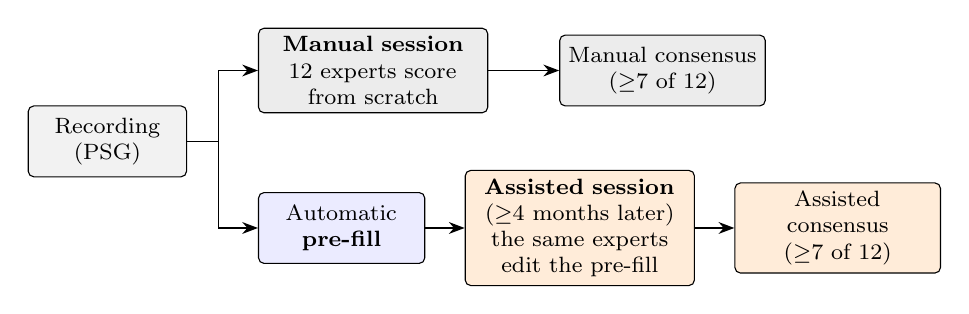
\begin{tikzpicture}[font=\footnotesize,
  box/.style={draw, rounded corners=2pt, align=center, minimum height=9mm, inner sep=3pt, text width=#1},
  box/.default=27mm, arr/.style={-{Stealth[length=2mm]}, semithick}]
\node[box=18mm, fill=gray!10] (psg) {Recording\\(PSG)};
\node[box, right=9mm of psg, yshift=9mm, fill=gray!15] (man) {\textbf{Manual session}\\12 experts score from scratch};
\node[box=19mm, right=9mm of psg, yshift=-11mm, fill=blue!8] (auto) {Automatic\\\textbf{pre-fill}};
\node[box, right=5mm of auto, fill=orange!15] (semi) {\textbf{Assisted session}\\($\ge$4 months later) the same experts edit the pre-fill};
\node[box=24mm, right=9mm of man, fill=gray!15] (cm) {Manual consensus\\($\ge$7 of 12)};
\node[box=24mm, right=5mm of semi, fill=orange!15] (cs) {Assisted consensus\\($\ge$7 of 12)};
\draw[arr] (psg.east) -- ++(4mm,0) |- (man.west);
\draw[arr] (psg.east) -- ++(4mm,0) |- (auto.west);
\draw[arr] (auto) -- (semi);
\draw[arr] (man) -- (cm);
\draw[arr] (semi) -- (cs);
\end{tikzpicture}
\caption{Design. PSG-IPA provides, for each recording, 12 manual scorings, 12 assisted scorings by the same experts,
and the pre-fill that the assisted scorings started from. Five recordings are provided for each of four tasks.
\textbf{Anchoring:} each expert's agreement with the pre-fill, assisted minus manual. \textbf{Inflation:} the
pre-fill's agreement gain from the manual to the assisted consensus, minus the gain of each expert's manual scoring
against the other 11 experts' consensus. \textbf{Independent algorithms:} two sleep stagers that no expert saw, judged
against both consensuses.}
\label{fig:design}
\end{figure}

\subsection{Primary measures and inference}

\textbf{Anchoring.} For expert $s$ and recording $r$,
\begin{equation}
\dA(s,r) = \mathrm{agr}\bigl(\mathrm{assisted}(s,r),\,\mathrm{prefill}(r)\bigr) - \mathrm{agr}\bigl(\mathrm{manual}(s,r),\,\mathrm{prefill}(r)\bigr).
\end{equation}
Positive values mean that the expert's assisted scoring lies closer to the pre-fill than their manual scoring.

\textbf{Reference inflation.} For each recording, $\dauto$ is the change in the pre-fill's agreement from the manual
to the assisted consensus, and $\dhuman$ is the same change for each expert's manual scoring, judged against the other
11 experts' assisted minus manual consensus and averaged over the 12 experts. If assistance only made the reference more accurate, these raters, who had not seen the pre-fill, would gain about
as much as the algorithm, and the difference in differences, $\mathrm{DiD}=\dauto-\dhuman$, would be close to zero. Because each
expert's manual scoring shares its session with the manual consensus, any difference between sessions unrelated to the
pre-fill also lowers $\dhuman$, so we interpret the DiD as inflation relative to session-matched raters; the
independent algorithms below have no session.

\textbf{Inference.} The units were the 20 recording-task combinations. The primary tests were exact two-sided sign
tests over these units ($\alpha=0.05$), applied to the recording-level mean of $\dA$ and to the DiD. Because all units share the same 12 experts, the tests support conclusions about these experts on these
recordings only. Per-task means come with 95\% crossed-bootstrap intervals that resample experts and recordings
independently \citep{owen2007}; with five recordings per task they are descriptive. The many secondary sign tests and intervals are unadjusted and are read as descriptions, not separate
confirmations. The pre-specified decision rule called the result positive if both sign tests were significant in the positive
direction and at least one task had a mean $\dA$ of 0.05 or more, a threshold set by judgment.

\subsection{Secondary analyses}

We computed pairwise percent agreement among the 12 scorings of each session where the pre-fill agreed with the
manual consensus and where it disagreed, events per hour of sleep for the pre-fill and both consensuses, and the
\emph{acceptance lift}: the probability that an assisted label equals the pre-fill's label minus the same probability
for the manual label. The lift was computed by the stage the pre-fill assigned, by how many of the 12 manual scorings
shared the most frequent label, and on labels that most experts had rejected: units where at least 9 of the other 11
experts' manual labels differed from the pre-fill's; selecting them without the scored expert's own label avoids the
regression to the mean of the first amendment's rule (at least 10 of 12, the scored expert included), and for events
the units were whole pre-fill events, adopted when an expert's scoring overlapped them.
\emph{Side-taking} compares, among units where both consensuses exist and differ, the share where the assisted
consensus equals the pre-fill with the share where the manual consensus does (equal if the sessions were
exchangeable; exact sign test over the 20 units). Anchoring was also computed for apneas and hypopneas separately, and the primary tests were repeated under four
robustness variants and with consensus events shorter than the rules' minimum durations dropped (Supplementary
Methods).

Two other stagers, independent of the pre-fill and never shown to any expert, scored each sleep-staging recording with
their default pretrained models:
YASA 0.7.0 \citep{vallat2021} and GSSC 0.0.9 \citep{hanna2023}, using the C4-M1 EEG (Cz-M1 in one recording) and
E1-M2 electrooculogram channels (YASA also chin electromyography). The protocol named YASA, the last amendment added GSSC, and their settings were fixed before they were run. For
each stager we report kappa against both consensuses and the pre-fill's lead over it (the pre-fill's kappa minus the
stager's against the same consensus); the lead over GSSC was pre-specified, the lead over YASA was an exploratory
addition to the protocol's YASA check. Because
an assisted
panel reaches a consensus on more hard epochs, which alone lowers an independent rater's measured agreement, changes
were also computed on epochs where both consensuses exist (\emph{common support}). As a negative control, on epochs
where a stager and the pre-fill disagreed, we computed each expert's movement toward the stager's label and toward
the pre-fill's (assisted minus manual share of matching labels); a general shift toward algorithm-like or more
typical scoring would move experts toward the stagers too.

A two-label latent-class model calibrated to the staging data illustrated how anchoring propagates into references of
different sizes and rules; its truth is, by construction, what a large unassisted panel would converge to, and its
outputs are illustrations, not estimates (Supplementary Methods).

\subsection{Unassisted audit}

We emulated a validation that scores every epoch with assistance and has the same experts score a random sample of
30-minute blocks without the pre-fill, drawn within each recording. We compared four estimates of an algorithm's
agreement with the unassisted consensus: the assisted consensus alone; a 9-of-12 assisted consensus; the audited blocks
alone; and a \emph{difference estimator} (prediction-powered inference \citep{angelopoulos2023}), which adds the mean,
over audited epochs, of the unassisted minus the assisted agreement to the mean assisted agreement over all epochs. The
targets were the pre-fill's and YASA's percent agreement and their gap, on the \val{c4-pop} sleep-staging epochs
(\val{c4-blocks} blocks) where both algorithms are labelled and the manual consensus exists, with exact design-based
standard errors \citep{cochran1977} and the large-sample multiplier (Supplementary Table~\ref{tab:s-blocks} also
gives the $t$-multiplier values for the audit's own degrees of freedom). The emulation's unassisted labels come from the earlier session, a best case for a
real audit; single-epoch audits, though impractical, are reported for comparison.

\subsection{How FDA-cleared devices built their references}

We reviewed every 510(k) clearance by the U.S. Food and Drug Administration (FDA) under product code OLZ (automatic
event detection software for polysomnography with EEG) listed by the openFDA device interface \citep{fda510k}:
\val{fda-census} clearances up to \val{fda-last-date}. Devices cleared under other product codes, for example
sleep-scoring systems cleared as polysomnographs, were not reviewed. For the \val{fda-modern} clearances since \val{fda-first-year},
we coded from each public summary how the reference for clinical performance testing was produced, how many scorers
were involved, whether the summary stated that the scorers were blinded to the device's output, and whether it said
that they had worked from automatic pre-scoring by any software, recording the verbatim passage behind every code. A
reference described only as manually scored was not counted as a statement about pre-scoring, because manual scoring
can be done in software that pre-scores automatically.
The AI assistant named in the statement on generative AI coded the first three fields; one of two authors checked them
against each summary and recorded the fourth, pre-scoring, during that check; the assistant confirmed their four
corrections against the cited passages. The two checkers then re-coded the three key fields of all \val{fda-perf}
summaries by hand without seeing any code, each blind for the summaries the other had checked; a third author settled
disagreements from the summary text (Supplementary Methods).
Summaries are abbreviated, so we report what they state, not what the submissions contained.

% =====================================================================
\section{Results}

\subsection{Assisted scorings were closer to the pre-fill}

Assisted scorings lay closer to the pre-fill than the same experts' manual scorings in \val{m1-sign-pos} of 20
recording-task units ($p=\val{m1-sign-p}$; Table~\ref{tab:primary}, Figure~\ref{fig:primary}a; Supplementary Table~\ref{tab:s-units}). Task means ranged
from \val{m1-task-min} to \val{m1-task-max}, and \val{m1-scorers-pos-min} to \val{m1-scorers-pos-max} of the 12
experts shifted toward the pre-fill in each task; the one unit without a shift, an arousal recording, was at
\val{m1-unit-min}. By the pre-specified decision rule, the result is positive, and it held under every robustness
variant (Supplementary Table~\ref{tab:s-r6}).

\begin{table}[tbp]
\centering
\footnotesize
\caption{Primary results by task. Agreement is Cohen's kappa for sleep stages and event F1 for the event tasks.}
\label{tab:primary}
\begin{adjustbox}{max width=\linewidth}
\begin{tabular}{lccccc}
\toprule
Task & \makecell{Anchoring $\Delta A$\\(95\% interval)} & \makecell{Experts\\$>0$} & \makecell{$\Delta_{\mathrm{auto}}$\\range} & \makecell{$\Delta_{\mathrm{human}}$\\range} & \makecell{Inflation DiD\\(95\% interval)} \\
\midrule
Sleep stages & \makecell{0.081\\(0.038 to 0.129)} & 11/12 & +0.056 to +0.102 & \ensuremath{-}0.022 to \ensuremath{-}0.011 & \makecell{0.091\\(0.072 to 0.112)} \\
EEG arousals & \makecell{0.066\\(0.011 to 0.133)} & 10/12 & +0.018 to +0.155 & \ensuremath{-}0.043 to +0.004 & \makecell{0.089\\(0.042 to 0.145)} \\
Respiratory events & \makecell{0.129\\(0.059 to 0.207)} & 11/12 & +0.034 to +0.255 & \ensuremath{-}0.132 to \ensuremath{-}0.012 & \makecell{0.178\\(0.066 to 0.300)} \\
Limb movements & \makecell{0.103\\(0.066 to 0.144)} & 12/12 & +0.015 to +0.094 & \ensuremath{-}0.016 to +0.001 & \makecell{0.054\\(0.023 to 0.089)} \\
\bottomrule
\end{tabular}
\end{adjustbox}
\par\smallskip
\begin{minipage}{0.95\linewidth}\footnotesize Anchoring: assisted minus manual agreement of the same expert with the pre-fill, averaged over 12 experts and 5 recordings. Experts $>0$: the number of the 12 experts whose mean anchoring over the task's recordings is positive. $\Delta_{\mathrm{auto}}$: change in the pre-fill's agreement from the manual to the assisted consensus; $\Delta_{\mathrm{human}}$: the same change for each expert's manual scoring against the other 11 experts' consensus (ranges over the 5 recordings). DiD $=\Delta_{\mathrm{auto}}-\Delta_{\mathrm{human}}$. Intervals are crossed-bootstrap intervals over experts and recordings and are descriptive. Exact sign tests over the 20 recording-task units: anchoring positive in 19/20 ($p=\ensuremath{4.0\times10^{-5}}$), inflation in 20/20 ($p=\ensuremath{1.9\times10^{-6}}$).\end{minipage}
\end{table}


\begin{figure}[tbp]
\centering
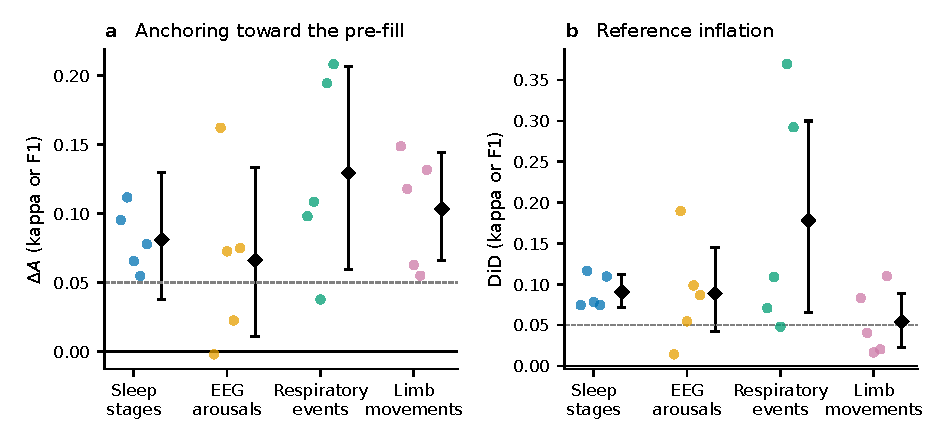
\includegraphics[width=\linewidth]{figures/fig_primary.pdf}
\caption{Primary results. (a) Anchoring: each expert's assisted minus manual agreement with the pre-fill, averaged
over experts, for each recording (dots). (b) Reference inflation: the pre-fill's agreement gain from the manual to
the assisted consensus, minus the gain of the same experts' manual scorings judged against the other experts'
consensus. Diamonds show task means with 95\% crossed-bootstrap intervals. The dashed line marks the pre-specified
material effect of 0.05.}
\label{fig:primary}
\end{figure}

\subsection{The references moved toward the pre-fill}

The two consensuses differed on a minority of units (\val{a2-stages-share} of common-support staging epochs); where
they did, the assisted consensus equaled the pre-fill in
\val{a2-min-pct} (arousals) to \val{a2-max-pct} (limb movements) of the changed units (epochs for stages, 0.1-second
bins for events), while the manual consensus rarely did (Figure~\ref{fig:mechanism}c; for
stages, \val{a2-stages-assisted} against \val{a2-stages-manual} over \val{a2-stages-n} changed epochs); the difference was
positive in \val{a2-sign-pos} of 20 units ($p=\val{a2-sign-p}$). Against the assisted rather than the manual consensus, the pre-fill's agreement rose in every unit
($\dauto>0$ in \val{m2-auto-units-pos} of 20, a gain with no session-matched baseline), while the experts' manual
scorings gained at most \val{m2-human-unit-max}, so the session-matched DiD was positive in \val{m2-sign-pos} of 20 units
($p=\val{m2-sign-p}$; Figure~\ref{fig:primary}b), and in all
\val{c6-sign-n} event units when consensus events shorter than the rules' minimum durations were dropped. On epochs
where both consensuses exist (sleep stages), the human raters' loss shrank to \val{a1-human-kappa-mean} kappa (95\% interval
\val{a1-human-kappa-lo} to \val{a1-human-kappa-hi}), while the pre-fill's own gain stayed positive in all
\val{c3-auto-kappa-pos} staging recordings (mean \val{c3-auto-kappa-mean}; common-support DiD \val{c3-did-kappa-mean}).
Judged against the assisted consensus, the experts' own manual consensus (\val{a3-stage-manual} for stages) was
closer than the pre-fill (\val{a3-stage-prefill}), the pre-fill being closer in \val{a3-units-pos} of \val{a3-units-n}
units, contrary to a pre-specified prediction (Supplementary Table~\ref{tab:s-predictions}): the assisted reference
remained predominantly the experts' own judgment.

\subsection{Where the pull arose}

The pull concentrated where experts disagree (Figure~\ref{fig:mechanism}a; Supplementary Tables~\ref{tab:s-r1r2}
and~\ref{tab:s-r3r4}). In every task the acceptance lift was near zero where all 12 experts had agreed manually and rose steadily as
manual agreement fell, reaching \val{r3-arousals-le7-mean} to \val{r3-limb-le7-mean}
across tasks where 7 or fewer agreed. Among stages it was largest for N1 (\val{r1-n1-mean}; 95\% interval \val{r1-n1-lo} to
\val{r1-n1-hi}), and N2 (\val{r1-n2-mean}) was the only stage whose descriptive interval included zero; for respiratory events,
anchoring was larger for hypopneas (\val{r2-hypopnea-mean}) than for apneas (\val{r2-apnea-mean}). These are the categories on which scorers agree least \citep{rosenberg2013,rosenberg2014,dankerhopfe2009}.

Experts also adopted labels that most colleagues had rejected: where at least 9 of the other 11 experts' manual
labels rejected the pre-fill's, the lift was \val{c1-stages-mean} for stages (95\% interval \val{c1-stages-lo}
to \val{c1-stages-hi}) and \val{c1-resp-mean} to \val{c1-limb-mean} for the event tasks, positive in \val{c1-sign-pos}
of 20 units and zero in the other ($p=\val{c1-sign-p}$ over the \val{c1-sign-nonzero} nonzero units;
Figure~\ref{fig:mechanism}b). The first amendment's rule,
which selects with the expert's own label, gave \val{r4-stages-mean} for stages. Where the pre-fill agreed with the manual consensus, assistance raised the experts' agreement with each other;
where it disagreed, agreement fell in three of four tasks (stages: \val{m3-stages-disagree-manual} to
\val{m3-stages-disagree-semi}; Supplementary Table~\ref{tab:s-m3}), as some experts followed the pre-fill and others
did not.

\begin{figure}[tbp]
\centering
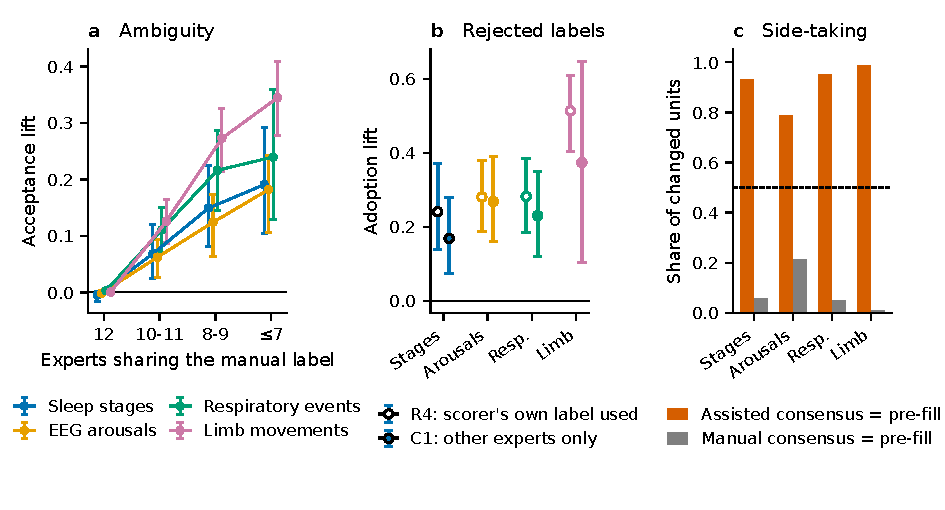
\includegraphics[width=\linewidth]{figures/fig_mechanism.pdf}
\caption{Where the pull arose. (a) Acceptance lift (probability that the assisted label equals the pre-fill, minus the
same probability for the manual label), by the number of the 12 experts who shared the most frequent manual label.
(b) The same lift on labels that most experts rejected manually, with units selected using the scored expert's own
label (open) or the other 11 experts' labels only (filled; events counted per event). Error bars are 95\%
crossed-bootstrap intervals. (c) Side-taking: among units where the two consensuses differ, the share where each
consensus equals the pre-fill. The dashed line marks equal shares.}
\label{fig:mechanism}
\end{figure}

\subsection{Algorithms the experts never saw}

YASA and GSSC disagreed with the pre-fill on \val{c2-yasa-differ} and \val{c2-gssc-differ} sleep-stage epochs. On
these epochs the experts' assisted labels moved toward the pre-fill (\val{c2-yasa-toward-prefill} and
\val{c2-gssc-toward-prefill}) and away from the stagers (\val{c2-yasa-toward-stager}, 95\% interval
\val{c2-yasa-toward-stager-lo} to \val{c2-yasa-toward-stager-hi}, and \val{c2-gssc-toward-stager}), in every recording
(Figure~\ref{fig:stagers}a; Supplementary Table~\ref{tab:s-stagers}). Where the two consensuses differed on such
epochs, the assisted consensus never took the stager's label, whereas the manual consensus took it in
\val{c2-yasa-side-manual-pct} (YASA) and \val{c2-gssc-side-manual-pct} (GSSC) of epochs.

Against the assisted consensus, both stagers lost agreement in four of five recordings while the pre-fill gained
(Table~\ref{tab:stagers}). The pre-fill's lead over YASA (exploratory) grew from \val{st-yasa-lead-manual-mean} to
\val{st-yasa-lead-assisted-mean} kappa and over GSSC from \val{st-gssc-lead-manual-mean} to
\val{st-gssc-lead-assisted-mean}: GSSC agreed better than the pre-fill with the manual consensus in \val{st-gssc-ahead-manual} of 5 recordings and
worse with the assisted consensus in all five (Figure~\ref{fig:stagers}b); on common support the growth of the lead,
which needs no human baseline, was positive in all five recordings for both stagers (mean \val{c3-yasa-sf-kappa-mean}
and \val{c3-gssc-sf-kappa-mean} kappa).

\begin{table}[tbp]
\centering
\footnotesize
\caption{Two independent stagers that no expert saw, judged against the manual and the assisted consensus (sleep stages, kappa).}
\label{tab:stagers}
\begin{adjustbox}{max width=\linewidth}
\begin{tabular}{lccccc}
\toprule
Recording & \makecell{YASA\\manual / assisted} & \makecell{GSSC\\manual / assisted} & \makecell{Pre-fill's lead over YASA\\manual / assisted} & \makecell{Pre-fill's lead over GSSC\\manual / assisted} & \makecell{$\Delta_{\mathrm{auto}}$,\\common support} \\
\midrule
SN1$^{a}$ & 0.812 / 0.821 & 0.818 / 0.830 & \ensuremath{-}0.024 / +0.029 & \ensuremath{-}0.029 / +0.020 & +0.043 \\
SN2 & 0.709 / 0.667 & 0.758 / 0.701 & +0.107 / +0.252 & +0.058 / +0.218 & +0.076 \\
SN3 & 0.753 / 0.706 & 0.865 / 0.847 & +0.101 / +0.204 & \ensuremath{-}0.011 / +0.063 & +0.032 \\
SN4 & 0.795 / 0.739 & 0.841 / 0.821 & +0.107 / +0.227 & +0.062 / +0.145 & +0.046 \\
SN5 & 0.736 / 0.671 & 0.865 / 0.802 & +0.105 / +0.259 & \ensuremath{-}0.024 / +0.128 & +0.074 \\
Mean &  &  & +0.079 / +0.194 & +0.011 / +0.115 & +0.054 \\
\bottomrule
\end{tabular}
\end{adjustbox}
\par\smallskip
\begin{minipage}{0.95\linewidth}\footnotesize Lead: the pre-fill's kappa minus the stager's, against the same consensus; a negative lead means the stager agreed better. $\Delta_{\mathrm{auto}}$, common support: the pre-fill's change from the manual to the assisted consensus on epochs where both consensuses exist. $^{a}$No C4-M1 channel; both stagers used Cz-M1.\end{minipage}
\end{table}


\begin{figure}[tbp]
\centering
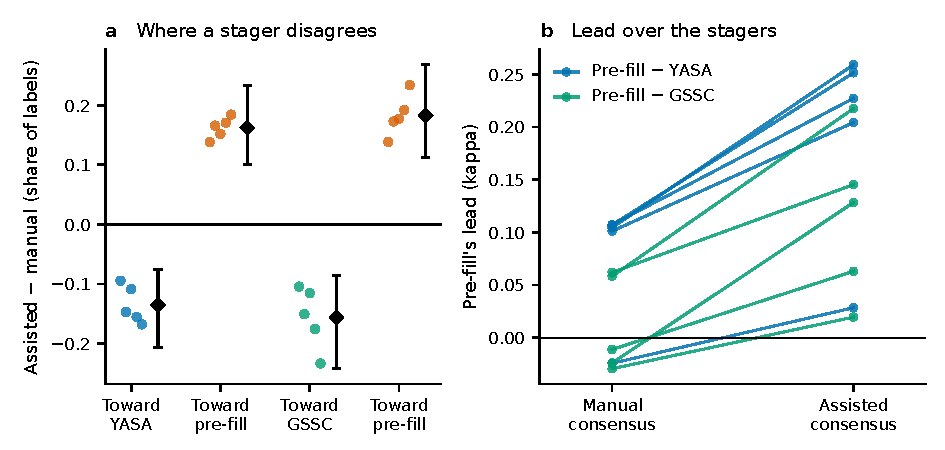
\includegraphics[width=\linewidth]{figures/fig_stagers.pdf}
\caption{Two sleep stagers that no expert saw. (a) On epochs where a stager and the pre-fill disagree, each expert's
assisted minus manual share of labels equal to the stager's and to the pre-fill's (dots: recordings; diamonds: means
with 95\% crossed-bootstrap intervals). (b) The pre-fill's lead in kappa over each stager, judged against the manual
and against the assisted consensus; each line is a recording.}
\label{fig:stagers}
\end{figure}

\subsection{Clinical indices}

The two consensuses differed by \val{m4-resp-diff-min} to \val{m4-resp-diff-max} respiratory events,
\val{m4-arousals-diff-min} to \val{m4-arousals-diff-max} arousals and \val{m4-limb-diff-min} to
\val{m4-limb-diff-max} limb movements per hour of sleep, and no recording changed its respiratory severity category
(Supplementary Table~\ref{tab:s-indices}). The pre-fill's index lay closer to the assisted than to the manual
consensus in \val{m4-resp-closer} of 5 respiratory and \val{m4-limb-closer} of 5 limb-movement recordings, but in
\val{m4-arousals-closer} of 5 arousal recordings, where assisted experts added arousals beyond those in the pre-fill.

\subsection{An unassisted audit of blocks}

On PSG-IPA (Table~\ref{tab:remedy}, Figure~\ref{fig:remedy}), the assisted reference overstated the pre-fill's
percent agreement with the unassisted consensus by \val{b1-prefill-d0-bias} and raised its lead over YASA from
\val{b1-gap-target} to \val{b1-gap-d0}. The 9-of-12 assisted reference overstated both further
(\val{b1-prefill-d0s-bias} and \val{b1-gap-d0s-bias}), because it keeps the epochs experts agree on, where the
pre-fill is nearly always right. When whole 30-minute blocks were audited, the difference estimator's 95\% half-width
for the lead fell below the assisted reference's bias from \val{c4-smallest-f} of blocks (\val{c4-gap-f10-share} of
epochs; half-width \val{c4-gap-f10-d2}, or \val{c4-gap-f10-d2-t-4dp} with the $t$ multiplier for 5 degrees of freedom, against a
bias of \val{c4-gap-bias-4dp});
single epochs needed 5\%, and the audited blocks alone needed more (Supplementary Table~\ref{tab:s-blocks}).

\begin{table}[tbp]
\centering
\footnotesize
\caption{Unassisted audits of 30-minute blocks, emulated on PSG-IPA (4{,}857 epochs in 87 blocks; percent agreement against the unassisted consensus).}
\label{tab:remedy}
\begin{adjustbox}{max width=\linewidth}
\begin{tabular}{lccccc}
\toprule
Quantity & \makecell{Unassisted\\target} & \makecell{Assisted reference\\(bias)} & \makecell{9-of-12 assisted\\(bias)} & \makecell{10\% of blocks\\D1 / D2} & \makecell{20\% of blocks\\D1 / D2} \\
\midrule
Pre-fill agreement & 0.898 & 0.947 (+0.048) & 0.975 (+0.077) & $\pm$0.098 / $\pm$0.024 & $\pm$0.062 / $\pm$0.016 \\
YASA agreement & 0.850 & 0.839 (\ensuremath{-}0.011) & 0.864 (+0.014) & $\pm$0.117 / $\pm$0.028 & $\pm$0.077 / $\pm$0.019 \\
Pre-fill minus YASA & 0.049 & 0.108 (+0.059) & 0.112 (+0.063) & $\pm$0.080 / $\pm$0.045 & $\pm$0.056 / $\pm$0.030 \\
\bottomrule
\end{tabular}
\end{adjustbox}
\par\smallskip
\begin{minipage}{0.95\linewidth}\footnotesize Audits draw whole blocks at random within each recording; 10\% of blocks hold 12\% and 20\% hold 21\% of the epochs. Audit columns give 95\% half-widths from exact formulas for stratified sampling of blocks, with the population variances and the large-sample multiplier, a known-variance best case (Supplementary Table~\ref{tab:s-blocks} gives the $t$-multiplier values). D1: the audited blocks alone; D2: the difference estimator combining them with the assisted consensus on all epochs. Both are unbiased by construction. Biases and half-widths are computed from unrounded values. Supplementary Table~\ref{tab:s-blocks} gives other audit sizes and the single-epoch audits.\end{minipage}
\end{table}


\begin{figure}[tbp]
\centering
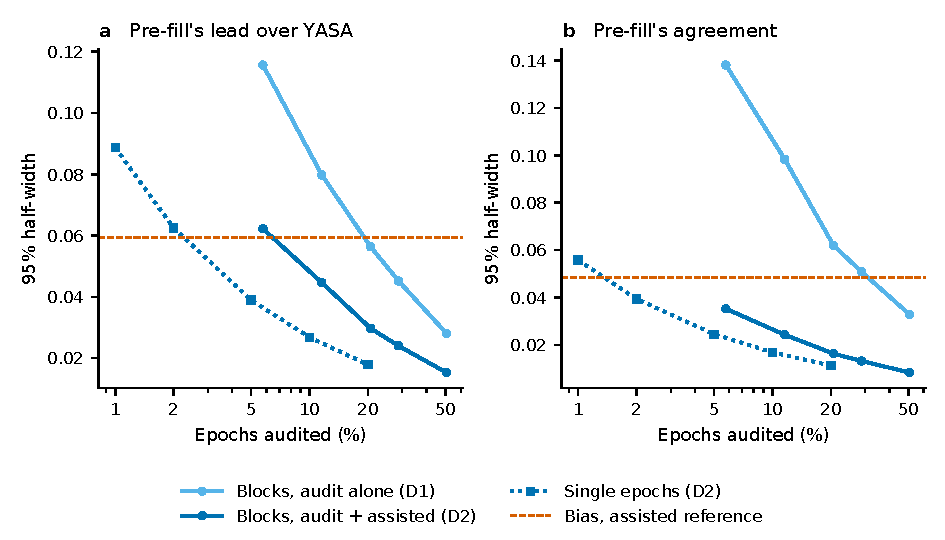
\includegraphics[width=\linewidth]{figures/fig_remedy.pdf}
\caption{Unassisted audits on PSG-IPA. 95\% half-widths of the audit estimates of (a) the pre-fill's lead over YASA
and (b) the pre-fill's agreement with the unassisted consensus, against the share of epochs audited: random 30-minute
blocks audited alone (D1) or combined with the assisted consensus by the difference estimator (D2), and single epochs
(D2). The dashed line is the bias of the assisted reference.}
\label{fig:remedy}
\end{figure}

\subsection{How FDA-cleared devices built their references}

Of the \val{fda-modern} clearances under product code OLZ since \val{fda-first-year}, \val{fda-perf} reported clinical
performance data
(Supplementary Table~\ref{tab:s-fda}). Their references were experts scoring independently for the study in \val{fda-indep} (three scorers in
\val{fda-indep-three}), a consensus not described as independent in \val{fda-consensus}, routine clinical scoring in
\val{fda-routine}, a daily-practice panel in \val{fda-daily}, another cleared algorithm's unedited output in
\val{fda-algo}, and not described in \val{fda-notdesc}. No summary reported whether reference scorers had worked from automatic pre-scoring by any software
(\val{fda-manual-ref} called the reference manually scored, which the coding rule does not count), and only
\val{fda-blind-explicit} stated that they had no access to the device's own output.
Blinding to the device was implied by the design in \val{fda-blind-implied}, stated without an object in
\val{fda-blind-object}, not applicable in \val{fda-blind-na} and not addressed in \val{fda-blind-none}. In the
blind second coding, the coders agreed with the first coding on
\val{d1-agree-min} to \val{d1-agree-max} of \val{fda-perf} summaries per field (kappa \val{d1-kappa-min} to
\val{d1-kappa-max}); adjudicating the \val{d1-disagreements} disagreements changed \val{d1-changed} code, SomnoMetry's
reference, to not described (Supplementary Table~\ref{tab:s-d1-items}).

% =====================================================================
\section{Discussion}

In this dataset, references built by editing an algorithm's pre-scoring were closer to it than the same experts'
unassisted references, in all four tasks and most where experts disagreed. In a benchmark of a commercial autoscorer, a thorough review changed 11.6\% of the staging epochs and introduced a
bias toward one expert scorer \citep{choo2023}. The shift went toward the algorithm the experts saw and away from two they did not, and against the assisted
reference the pre-fill outscored a stager that had matched it against the experts' unassisted judgment.

\textbf{What the data establish.} Our design cannot settle whether assistance made the references more or less accurate, since the truth is unknown. Against the standard we used,
the same experts' unassisted judgment, an assisted reference lies closer to the assisting algorithm, and two checks
narrow the alternatives. First, the shift was consistent with one specific to the algorithm shown: where two stagers that the
experts never saw disagreed with the pre-fill, the experts moved toward the pre-fill and away from both, so a general
drift between sessions toward more typical or algorithm-like scoring does not explain it; a drift toward this
center's conventions, on whose scorings the pre-fill's stager was developed and the other two were not, would produce
the same pattern and cannot be separated from anchoring in this design. Second, experts adopted labels that most colleagues had rejected, with the units selected without the experts' own
judgments; neither observation shows that the adopted labels were wrong. Many scoring decisions apply thresholds by eye, such as a limb movement's amplitude \citep{ferri2016} or a hypopnea's
desaturation,
and experts may share misses that a detector catches; the largest adoption lift (limb movements) and the larger
anchoring for hypopneas than for apneas are compatible with such corrections, whereas N1, which lacks a threshold of
the kind N3 and limb movements have and showed the largest stage lift, is where anchoring is the likelier reading. Keeping a pre-filled label costs nothing and changing it costs an action \citep{alvarezestevez2022}; ``anchoring''
here names the outcome, not a process. Planted-error experiments could separate the readings \citep{holm2025}. For the qualitative claim the distinction does not matter: a reference edited from one algorithm's output copies
its errors with its correct labels and cannot arbitrate between that algorithm and its competitors.

\textbf{Consequences for validation.} In our data the assisted reference overstated the pre-fill's percent agreement by \val{b1-prefill-d0-bias},
as much as its entire unassisted gap to YASA (\val{b1-gap-target}), and in kappa turned GSSC from level with the
pre-fill into trailing it in every recording. Because anchoring is a shared influence rather than independent noise,
adding experts does not remove it: in both model configurations a larger assisted majority converged on the pre-fill
(Supplementary Figure~\ref{fig:s-simulation}). A stricter consensus does not help either: it keeps the easy epochs and drops those where algorithms differ, and
in our data widened the pre-fill's lead. Clinical indices changed little and no severity category changed, so the clearest consequence concerns the
comparison and clearance of algorithms rather than diagnosis.

\textbf{How often could this reach practice?} In the OLZ clearances (other codes were not reviewed), the most common reference was experts scoring independently
for the study (\val{fda-indep} of \val{fda-perf}), a design that can exclude pre-scoring; in \val{fda-unclear} it was
routine clinical scoring, a daily-practice panel or not described, and no summary says whether
the scorers worked from pre-scoring. Where laboratory software pre-scores automatically, routine scoring may be assisted \citep{alvarezestevez2019}.

\textbf{Recommendations.} First, validation studies should report whether reference scorers saw any algorithm's
output, and which. STARD 2015 item 13b \citep{bossuyt2015}, the QUADAS-2 reference-standard domain \citep{whiting2011} and TRIPOD+AI
\citep{collins2024} already ask whether the reference was assessed without knowledge of the index test, which a
reference edited from the index algorithm's output answers in the negative by design, and the FDA's 2025 draft guidance on
AI-enabled devices asks how device outputs were blinded from the reference-standard determination \citep{fdaai2025};
pre-scoring by any software, and a reference built with one algorithm's help and used to judge another, the comparison
that in our data favored the assisting algorithm, are new items to report. The wording matters: ``computer-assisted scoring'' has meant both manual scoring in software
\citep{kuna2013,malhotra2013} and editing an automatic scoring \citep{punjabi2015}. Second, where assisted references are used, a random sample of 30-minute blocks, drawn and concealed in advance,
should be scored without assistance by scorers who have not seen the algorithm's labels, before the assisted
pass or by a separate panel that has not worked with the algorithm; every epoch of an audited block is re-scored, so
the software must withhold its pre-scoring there. In our data, auditing \val{c4-smallest-f} of blocks and combining the audit with the assisted reference
\citep{angelopoulos2023} estimated the algorithm's lead within \val{c4-gap-f10-d2}, less than the bias it corrects; the
fraction is this dataset's grid value (an audit elsewhere is sized so that its half-width falls below the smallest
difference that matters), and a real audit by experts who also work with the algorithm would be less independent. Asking each expert for a committed judgment before revealing the suggestion is an alternative; anchoring varied
widely between experts (Supplementary Table~\ref{tab:s-experts}), as automation-bias research would predict
\citep{parasuraman2010}. Third, references produced with one algorithm's assistance should not be used to compare it with others, and
datasets should document any pre-annotation and the model behind it \citep{gebru2021}, since reusing such labels to
train new models passes that algorithm's decisions on. The same applies to model-assisted imaging datasets \citep{dreizin2023,li2024} and to annotation with large
language models \citep{schroeder2025}.

\textbf{Limitations.} The data come from one center, with 12 experts, five recordings per task and one family of research pre-fill
algorithms by the dataset's authors; the pre-fill's stager was developed on this center's scorings and YASA and GSSC on cohorts
elsewhere, so part of the pre-fill's lead may be real, and commercial autoscoring, other
laboratories and scorers trained elsewhere may anchor more or less. The recordings sit at five percentiles of automatic-versus-clinical agreement (12.5th to 87.5th), so only the
tails, where the algorithm fails most, are unrepresented. The assisted session always came at least four months after the manual one (a randomized order would have been
better, as the dataset's creators noted \citep{alvarezestevez2022}), and whether these twelve experts used the algorithms in routine work before or between the sessions is not
documented; at center level the arousal detector's reviewed output had produced part of the clinical arousal
references before this dataset was scored (220 of 472 routine recordings \citep{alvarezestevez2019}), and the staging pre-fill comes from a stager developed on the center's clinical scorings
\citep{alvarezestevez2021}, which version is not documented. Exposure before the manual session makes the measured shift a lower bound; exposure between the sessions would
also move unassisted judgment toward the algorithm and inflate it. The negative control is consistent with a shift specific to the pre-fill rather than toward algorithm-like scoring
but cannot detect one toward conventions that only the pre-fill encodes, and the selection of rejected
labels assumes that experts label independently within a session. The clinical indices pool apneas and
hypopneas without a documented hypopnea rule. The plans were dated and hashed but not registered, and the protocol and first amendment were committed with
their results. The blind second coders were authors,
blind to the codes but not to the hypothesis. A prospective study with randomized session order, or a replication with planted errors \citep{holm2025}, would
address the open questions.

% =====================================================================
\section{Conclusions}

In this dataset, references built by editing an algorithm's pre-scoring were closer to that algorithm than the same
experts' unassisted scoring, and favored it over sleep stagers the experts never saw. Validations
should report how their references were made, not compare an algorithm against references built with its help, and
audit a random sample of blocks scored without assistance before any exposure to the algorithm's labels.

% =====================================================================
\bibliographystyle{unsrtnat}
\bibliography{references}

\end{document}
